% This is the Reed College LaTeX thesis template. Most of the work
% for the document class was done by Sam Noble (SN), as well as this
% template. Later comments etc. by Ben Salzberg (BTS). Additional
% restructuring and APA support by Jess Youngberg (JY).
% Your comments and suggestions are more than welcome; please email
% them to cus@reed.edu
%
% See http://web.reed.edu/cis/help/latex.html for help. There are a
% great bunch of help pages there, with notes on
% getting started, bibtex, etc. Go there and read it if you're not
% already familiar with LaTeX.
%
% Any line that starts with a percent symbol is a comment.
% They won't show up in the document, and are useful for notes
% to yourself and explaining commands.
% Commenting also removes a line from the document;
% very handy for troubleshooting problems. -BTS

% As far as I know, this follows the requirements laid out in
% the 2002-2003 Senior Handbook. Ask a librarian to check the
% document before binding. -SN

%%
%% Preamble
%%
% \documentclass{<something>} must begin each LaTeX document
\documentclass[12pt,twoside]{reedthesis}
% Packages are extensions to the basic LaTeX functions. Whatever you
% want to typeset, there is probably a package out there for it.
% Chemistry (chemtex), screenplays, you name it.
% Check out CTAN to see: http://www.ctan.org/
%%
\usepackage{graphicx,latexsym}
\usepackage{amsmath}
\usepackage{amssymb,amsthm}
\usepackage{longtable,booktabs,setspace}
\usepackage{chemarr} %% Useful for one reaction arrow, useless if you're not a chem major
\usepackage[hyphens]{url}
% Added by CII
\usepackage[hidelinks]{hyperref}
\usepackage{lmodern}
\usepackage{float}
\floatplacement{figure}{H}
% End of CII addition
\usepackage{rotating}

% Next line commented out by CII
%%% \usepackage{natbib}
% Comment out the natbib line above and uncomment the following two lines to use the new
% biblatex-chicago style, for Chicago A. Also make some changes at the end where the
% bibliography is included.
%\usepackage{biblatex-chicago}
%\bibliography{thesis}


% Added by CII (Thanks, Hadley!)
% Use ref for internal links
\renewcommand{\hyperref}[2][???]{\autoref{#1}}
\def\chapterautorefname{Chapter}
\def\sectionautorefname{Section}
\def\subsectionautorefname{Subsection}
% End of CII addition

% Added by CII
\usepackage{caption}
\captionsetup{width=5in}
% End of CII addition

% \usepackage{times} % other fonts are available like times, bookman, charter, palatino


% To pass between YAML and LaTeX the dollar signs are added by CII
\title{\textbf{\Huge{On the Numerical simulation of the \\[20pt] Heston model}}}
\author{Fernando O. Teixeira}
% The month and year that you submit your FINAL draft TO THE LIBRARY (May or December)
\date{setembro 22, 2017}
\division{Applied Mathematics}
\advisor{Hugo Alexander de la Cruz Cancino}
%If you have two advisors for some reason, you can use the following
% Uncommented out by CII
% End of CII addition

%%% Remember to use the correct department!
\department{Mathematics}
% if you're writing a thesis in an interdisciplinary major,
% uncomment the line below and change the text as appropriate.
% check the Senior Handbook if unsure.
%\thedivisionof{The Established Interdisciplinary Committee for}
% if you want the approval page to say "Approved for the Committee",
% uncomment the next line
%\approvedforthe{Committee}

% Added by CII
%%% Copied from knitr
%% maxwidth is the original width if it's less than linewidth
%% otherwise use linewidth (to make sure the graphics do not exceed the margin)
\makeatletter
\def\maxwidth{ %
  \ifdim\Gin@nat@width>\linewidth
    \linewidth
  \else
    \Gin@nat@width
  \fi
}
\makeatother

\renewcommand{\contentsname}{Table of Contents}
% End of CII addition

\setlength{\parskip}{0pt}

% Added by CII

\providecommand{\tightlist}{%
  \setlength{\itemsep}{0pt}\setlength{\parskip}{0pt}}

\Acknowledgements{
\textbf{\\ \\ \\ \\ \\ \\ \\ \\ \\ \\ \\ \\ \\ \\ \\ \\ \\ \\ \\ \\ \\ \\ \\ \\ \\ \\ \\ \\ \\ \\ \\ \\ \\ \\ \\ \\ \\ \\ \\ \\ \\ \\ \\ \\ \\ \\ \\ \\ \\ \\ \\ \\ \\ \\ \\ \\ \\ \\ \\ \\ \\ \\ \\ }
You get pseudo-order when you seek order; you only get a measure of
order and control when you embrace randomness. --- Nassim Nicholas Taleb
}

\Dedication{

}

\Preface{

}

\Abstract{
In this thesis we revisit some of the numerical methods for solving the
Heston model's European call. Specifically, we approach the Euler, the
Kahl-Jackel an two versions of the exact algorithm schemes. To perform
this task, firstly we present a literature review which brings
stochastic calculus, the Black-Scholes (BS) model and its limitations,
the stochastic volatility methods and why they resolve the issues of the
BS model, and the peculiarities of the numerical methods - convergence,
discretization and stability. Since it is impossible to have a deep
approach to all these topics, we provide recommendations when we
acknowledge that the reader might need more specifics. We introduce the
methods aforementioned providing all our implementations in R language.
Also, we deliver an R package with these functions and others.
\newline \newline \textbf{Keywords:} Heston, Stochastic, Volatility,
Black-Scholes, European call, R
}

	\usepackage{mathtools}
	\usepackage{cancel}
	\graphicspath{ {figure/} }
	\usepackage{enumitem}
	\usepackage{caption}
	\usepackage{graphicx}
% End of CII addition
%%
%% End Preamble
%%
%

\usepackage{amsthm}
\newtheorem{theorem}{Theorem}[section]
\newtheorem{lemma}{Lemma}[section]
\theoremstyle{definition}
\newtheorem{definition}{Definition}[section]
\newtheorem{corollary}{Corollary}[section]
\newtheorem{proposition}{Proposition}[section]
\theoremstyle{definition}
\newtheorem{example}{Example}[section]
\theoremstyle{remark}
\newtheorem*{remark}{Remark}
\let\BeginKnitrBlock\begin \let\EndKnitrBlock\end
\begin{document}

% Everything below added by CII
      \maketitle
  
  \frontmatter % this stuff will be roman-numbered
  \pagestyle{empty} % this removes page numbers from the frontmatter
      \begin{acknowledgements}
      \textbf{\\ \\ \\ \\ \\ \\ \\ \\ \\ \\ \\ \\ \\ \\ \\ \\ \\ \\ \\ \\ \\ \\ \\ \\ \\ \\ \\ \\ \\ \\ \\ \\ \\ \\ \\ \\ \\ \\ \\ \\ \\ \\ \\ \\ \\ \\ \\ \\ \\ \\ \\ \\ \\ \\ \\ \\ \\ \\ \\ \\ \\ \\ \\ }
      You get pseudo-order when you seek order; you only get a measure of
      order and control when you embrace randomness. --- Nassim Nicholas Taleb
    \end{acknowledgements}
  
      \hypersetup{linkcolor=black}
    \setcounter{tocdepth}{2}
    \tableofcontents
  
      \listoftables
  
      \listoffigures
      \begin{abstract}
      In this thesis we revisit some of the numerical methods for solving the
      Heston model's European call. Specifically, we approach the Euler, the
      Kahl-Jackel an two versions of the exact algorithm schemes. To perform
      this task, firstly we present a literature review which brings
      stochastic calculus, the Black-Scholes (BS) model and its limitations,
      the stochastic volatility methods and why they resolve the issues of the
      BS model, and the peculiarities of the numerical methods - convergence,
      discretization and stability. Since it is impossible to have a deep
      approach to all these topics, we provide recommendations when we
      acknowledge that the reader might need more specifics. We introduce the
      methods aforementioned providing all our implementations in R language.
      Also, we deliver an R package with these functions and others.
      \newline \newline \textbf{Keywords:} Heston, Stochastic, Volatility,
      Black-Scholes, European call, R
    \end{abstract}
  
  \mainmatter % here the regular arabic numbering starts
  \pagestyle{fancyplain} % turns page numbering back on

  \newcommand{\source}[1]{\caption*{Source: {#1}} }
  
  
  
  \chapter{Introduction}\label{intro}
  
  The french mathematician Louis Bachelier was the trail-blazer that
  brought Brownian motion, previously restricted to the field of botanics
  where it was firstly observed, to the financial framework. He modeled
  the stock prices as a Brownian motion with drift. In 1973, Black and
  Scholes {[}1{]} designed a model based on the Geometric Brownian Motion
  to price options.
  
  Options are derivatives that give their bearers the rights to buy or
  sell a specific asset in a future date and with a predetermined price.
  They are, by design, affected by small variations in the underlying
  assets' components, for example, the variance.
  
  The Black-Scholes model was once the standard way of option pricing, but
  was replaced by more modern models that are now prevalent. One of the
  main drawbacks of the Black-Scholes model is the strong assumption that
  the stock returns' volatility is constant. Thus, the implied model's
  volatility results in a flat surface when plotted against the option's
  strike price and maturity. Real world implied volatility varies with the
  strike price and maturity, forming what is called the `volatility
  smile'.
  
  The Heston model is an extension of the Black-Scholes model that tackles
  this volatility issue replacing the constant volatility with a
  stochastic process. There are many models that approach volatility
  stochastically, but the Heston has valuable characteristics such as
  presenting an analytical solution to the option pricing and also having
  a computationally simple implementation when compared to more
  sophisticated competitors.
  
  We aim with this thesis to better understand the Heston model, its
  quirkinesses, associated numerical methods and their implementations,
  and eventually discuss its pros and cons. For such, we will not only
  discuss the challenges in a vaguely way, but show code snippets of our
  implementations in R programming language {[}2{]} to help clarify
  possible associated difficulties. Furthermore, since we didn't find code
  for the exact algorithm implementation we intend to release a CRAN
  package with the codes as a didactic tool.
  
  This thesis is divided into five chapters, the first being this
  introduction. Following, we have a literature review that mainly
  addresses stochastic calculus, the Black-Scholes models and the Heston
  model. Thereafter we present the different Heston model implementations.
  Chapter 4 brings the results of the tests we perform and finally,
  chapter 5 presents the conclusion and work limitations.
  
  \chapter{Theoretical Framework}\label{lt-review}
  
  This chapter presents the concepts of stochastic calculus, from the
  historic conception of how it first arose through the basic principles
  and applications in finance. We address with more care the classical
  Black-Scholes model and its limitations and the Heston model. This model
  is also well known, it brings the concept of stochastic volatility in
  it, which brings its results closer to reality.
  
  \section{Stochastic Calculus}\label{stochastic-calculus}
  
  Stochastic calculus arises from stochastic processes and allows the
  creation of a theory of integration where both the integrand and
  integrator terms are stochastic processes. Stochastic calculus was
  created by the Japanese mathematician Kiyosi Itô
  \footnote{There is another important stochastic integral, called the \textit{Stratonovich Integral} that unlike the Itô's integral, respects the conventional calculus chain rule. Also, the integral is evaluated at the interval's midpoint, instead of its left extreme. A Stratonovich integral can be expressed as an Itô integral and vice versa.}
  in the 1940s and 1950s and is used for modeling financial options and in
  another wide variety of fields {[}3{]}. In this chapter we present the
  historical contexts in which the tools and models are used, but our
  focus is introducing the concepts and notations that will be further
  used in our work.
  
  \subsection{Stochastic differential equation -
  SDE}\label{stochastic-differential-equation---sde}
  
  At first, before introducing stochastic differential equation, it is
  helpful to start with ordinary differential equation. Let \(x_t\) denote
  an asset at time \(t\) so that the change in the asset at time \(t\) is
  given by the following deterministic differential equation:
  \begin{align}
  dx_t &= f(t, x_t)dt \\
  x(0) &= x_0 \nonumber
  \end{align}
  We now add a ``noise'' to this equation:
  \begin{align} \label{eq:sde1}
  dx_t &= \overbrace{\underbrace{f(t, x_t)}_\text{drift}dt}^\text{deterministic} + \overbrace{\underbrace{g(t, x_t)}_\text{diffusion}dW_t}^\text{random shock} \\
  x(0) &= x_0 \nonumber
  \end{align}
  This ``noise'' \(dW_t\) is a \emph{random} Wiener process (which will be
  clarified below) and \(x_0\) is our initial value.
  
  The \(g(t, x_t)\) part of the SDE is often referred as \emph{diffusion
  coefficient}, these usually have a continuous paths. Before moving on,
  we must carefully define what the term \emph{random} means and the best
  way to begin doing so is to precisely define a probability space:
  
  \BeginKnitrBlock{definition}[Probability Space]
  
  \protect\hypertarget{def:unnamed-chunk-1}{}{\label{def:unnamed-chunk-1}
  \iffalse (Probability Space) \fi{} }A triple (\(\Omega\),
  \(\mathcal {U}\), \(\mathcal {P}\)) is called a
  \textit{probability space} provided \(\Omega\) is any set,
  \(\mathcal {U}\) is a \(\sigma\)-algebra of subsets of \(\Omega\) and
  \(\mathcal {P}\) is a probability measure on \(\mathcal {U}\) .
  
  \EndKnitrBlock{definition}
  
  \subsection{Brownian Motion}\label{brownian-motion}
  
  The Brownian motion is the name given to the irregular motion observed
  in the motion of pollen particles suspended in fluid resulting from
  particle collision with atoms or molecules. It is named after Robert
  Brown, the first to have observed the movement in 1828. He noted two
  characteristic in the pollen movement {[}3{]}:
  \begin{itemize}
  \item
    the path of a given particle is very irregular, having a tangent at no
    point
  \item
    the motion of two distinct particles appear to be independent
  \end{itemize}
  The first quantitative works in Brownian motion come from an interest in
  stock price fluctuation by Bachelier in 1900. Albert Einstein also
  leaned over the subject and in 1905 derived the transition density for
  Brownian motion from molecular-kinetic theory of heat {[}3,4{]}.
  
  In 1923, the Wiener process was coined in honor of Norbert Wiener
  mathematical proof of existence of the Brownian motion and stating its
  properties.\footnote{More can be found on {[}5--7{]}.}
  
  \BeginKnitrBlock{definition}[Wiener Process]
  
  \protect\hypertarget{def:unnamed-chunk-2}{}{\label{def:unnamed-chunk-2}
  \iffalse (Wiener Process) \fi{} }Given a probability space (\(\Omega\),
  \(\mathcal {U}\), \(\mathcal {P}\)), a stochastic process \(W_t\)
  defined in this space is a \emph{Wiener process} if it satisfies the
  following properties:
  \begin{itemize}
    \item  $W_{0}=0$
    
    \item The change in $W$, given by $\Delta W = W_{t+\Delta t}-W_{t}$, is normally distributed with mean zero and standard deviation $\sqrt{\Delta t}$, meaning that $\Delta W = \epsilon\sqrt{\Delta t}$, where $\epsilon$ is $N(0,1)$.
    
    \item If the increment $\Delta t_1$ does not overlap with the time increment $\Delta t_2$, then $\Delta W_1$ and $\Delta W_2$ are independent.
    
    \item The process is continuous, meaning that there are no jumps in the path.
    
    \item The process is Markovian. This means that the conditional expectation of $W_{t+1}$ given its entire history is equal to the conditional expectation of $W_{t+1}$ given today's information. This can be written as: $E[W_{t+1}|W_1, ..., W_t] = E[W_{t+1}|W_t]$.
    
    \item Consider the time interval $[0,t]$ with $n$ equally spaced intervals given by $t_i = \frac{it}{n}$. Then the paths of the Brownian motion have unbounded variation, this means that they are not differentiable and go towards infinity as $n$ increases. The quadratic variation is given by $\sum_{i=1}^{n}{(Z_{t_i}-Z_{t_{i-1}})^2} \rightarrow t$, meaning that when $n$ increases it stays constant at $t$. 
  
  \end{itemize}
  \EndKnitrBlock{definition}
  \begin{figure}
  
  {\centering 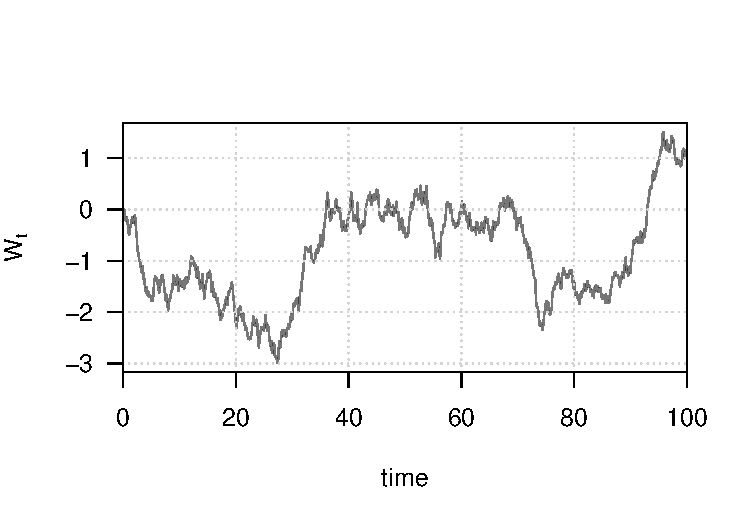
\includegraphics{thesis_files/figure-latex/wiener-1} 
  
  }
  
  \caption{A Wiener process trajectory path example \label{wiener}}\label{fig:wiener}
  \end{figure}
  \subsubsection{Correlated Brownian Motions}\label{corr}
  
  Two independent Brownian motions that are correlated can describe a new
  process \(Z_t\). Let \(W_1\) and \(W_2\) be these two \emph{independent}
  Brownian motions and let \(-1 \leq \rho \leq 1\) be a given number. For
  \(0 \leq t \leq T\) define the new process \(Z_t\) as {[}3{]}:
  \begin{align}
  \label{eq:corr_brow}
  Z_t = \rho W_{1,t} + \sqrt{1-\rho^2}W_{2,t}
  \end{align}
  \noindent
  This equation is a linear combination of independent normals at each
  timestep \(t\), so \(Z_t\) is normally distributed. It is proven that
  \(Z\) is a Brownian motion and that \(Z\) and \(W_{1,t}\) have
  correlation \(\rho\) {[}3{]}.
  
  \subsection{Itô's Integral}\label{itos-integral}
  
  Formally, the SDE presented in equation \eqref{eq:sde1} is interpreted as
  {[}6--11{]}:
  \begin{align} 
  \label{eq:sde2}
  x_t &= x_0 + \int_{0}^{t}{f(s, x_s)ds} + \int_{0}^{t}{g(s, x_s)dW_s}
  \end{align}
  \noindent
  for some \(f(s, x_s)\), \(g(s, x_s)\) and \(s \in [0,t]\).
  
  The Itô integral can, as the Riemann integral, be approximated by a
  finite sum. Also, it has a definition as a certain limit. Itô's lemma
  \ref{lem:itolemma} plays the same role as the fundamental theorem of
  calculus in allowing to evaluate integrals. It is the formal definition
  and presents an extra term not encountered in the conventional calculus
  theorem that is due to the non-smoothness characteristics of Brownian
  motion paths. It is possible, though, to define the integral in a less
  rigorous way:
  \begin{align}
  Y_{\Delta t}(t) \approx \sum_{t_k < t}{g(t_k)\Delta W_k}
  \end{align}
  \noindent
  with the usual notions \(t_k = k\Delta t\), and
  \(\Delta W_k = W(t_{k+1})-W(t_k)\). And in a more rigorous form, if the
  limit exists, then the Ito integral is:
  \begin{align}
  Y(t)  = \lim\limits_{\Delta t \to 0} Y_{\Delta t}(t)
  \end{align}
  It is essential that the \emph{forward difference} is used rather than
  the backward difference, which would be wrong.
  
  \BeginKnitrBlock{lemma}[Itô's Lemma]
  
  \protect\hypertarget{lem:itolemma}{}{\label{lem:itolemma} \iffalse (Itô's
  Lemma) \fi{} } Assume that \(S_t\) has a stochastic differential given
  by:
  \begin{align}
  dS_t = \mu_t dt + \sigma_t dW_t 
  \end{align}
  \noindent
  for \(\mu_t\), \(\sigma_t\) and \(t \in [0,T]\). Assume
  \(u: \mathbb{R} \times [0, T] \rightarrow \mathbb{R}\) is continuous and
  that \(\frac{\partial u}{\partial t}\),
  \(\frac{\partial u}{\partial x}\), \(\frac{\partial^2 u}{\partial x^2}\)
  exist and are continuous.
  \begin{align*}
  Y_t := u(S_t, t)
  \end{align*}
  \noindent
  Then Y has the following stochastic differential:
  \begin{align} 
  \label{eq:ito}
  \begin{split}
      dY_t &= \frac{\partial u}{\partial t}dt + \frac{\partial u}{\partial x} dS_t + \frac{1}{2}\frac{\partial^2 u}{\partial x^2}\sigma_t^2 dt  \\[10pt] 
      &= \left( \frac{\partial u}{\partial t} + \mu_t \frac{\partial u}{\partial x} + \frac{1}{2}\frac{\partial^2 u}{\partial x^2}\sigma_t^2 \right) dt + \sigma_t \frac{\partial u}{\partial x} dW_t
  \end{split}
  \end{align}
  \noindent  where the argument of \(u\),
  \(\frac{\partial u}{\partial x}\) and
  \(\frac{\partial^2 u}{\partial x^2}\) above is \(\left( S_t, t \right)\)
  .
  
  \EndKnitrBlock{lemma}
  
  Equation \eqref{eq:ito} is the stochastic equivalent to the chain rule,
  also known as Itô's formula or Itô's chain rule. The proof to this
  theorem is based on the Taylor expansion of the function \(f(S_t, t)\)
  {[}6,8{]}. For practical use you should write out a second-order Taylor
  expansion for the function to be analyzed and apply the multiplication
  table {[}3{]} presented in Table \ref{mat}.
  \begin{table}[ht]
  \centering
  \begin{tabular}{llr}
    \hline 
   & $dt$ & $dW_t$ \\ 
    \hline 
  $dt$ & 0 & 0 \\ 
    $dW_t$ & 0 & $dt$ \\ 
     \hline 
  \end{tabular}
  \caption{Box calculus} 
  \label{mat}
  \end{table}
  \subsubsection{Itô's Integral
  Properties}\label{itos-integral-properties}
  
  Let \(f\), \(g\) \(\in\) \(\mathcal{V}\) and let \(0 \leq t_0 < u < T\).
  Then
  \begin{enumerate}[label=(\roman*)]
    \item $\displaystyle \int_{t_0}^{T}{f dB_t} = \int_{t_0}^{u}{f dB_t} + \int_{u}^{T}{f dB_t}$
    \item $\displaystyle \int_{t_0}^{T}{(\alpha f + \beta g) dB_t} = \alpha  \int_{t_0}^{T}{f dB_t} + \int_{t_0}^{T}{ \beta g dB_t}$
    \item $\displaystyle \mathbb{E}\left[ \int_{t_0}^{T}{fdB_t}\right] = 0 $
    \item $\displaystyle \mathbb {E} \left[\left(\int_{0}^{t}H_{s}\,dB_{s}\right)^{2}\right]=\mathbb {E} \left[\int _{0}^{t}H_{s}^{2}\,ds\right]$ (Isometry)
    \item $ \displaystyle \mathbb {E}\left[ \int_{t_0}^{T}{f dB_t \mid \mathcal{F}_{s}} \right] = \int_{t_0}^{s}{f dB_t}, \,\,\,\,\,\,\,\,\,\,\,\,\,\, for \,\, s < T.$  (Martingale\footnote{A martingale is a stochastic process with certain characteristics. The main one is that the expected value in time $t+1$ for $X$ is the $X$ value in $t$. This means there are no winning strategies when we are dealing with martingales (unlike when we play poker, for example). A Wiener process is a martingale.})
  \end{enumerate}
  \section{Black-Scholes Model}\label{black-scholes-model}
  
  \subsection{Basics}\label{basics}
  
  The Black-Scholes (B-S) model arises from the need to price european
  options in the derivative markets. Derivatives are financial instruments
  traded in the market, stock exchange or over-the-counter (OTC) market,
  whose values depend on the values of an underlying asset. {[}1,12,13{]}
  \begin{itemize}
  \item
    A call option is a derivative that gives its bearer the right, but not
    the obligation, to purchase a specific asset by a fixed price before
    or on a given date.
  \item
    A put option is a derivative that gives its bearer the right, but not
    the obligation, to sell a specific asset by a fixed price before or on
    a given date.
  \end{itemize}
  The trading price of the option is called the option \emph{premium} and
  the asset from which the option derives is called the \emph{underlying
  asset}. This asset may be interest rates, exchange rates, stock
  exchanges indices, commodities or stocks. The fixed price in contract in
  which the underlying asset might to be bought or sold is the
  \emph{strick price}. The option expiration date is called the
  \emph{maturity}. {[}1,13{]}
  
  There are two major different option types: European and American. The
  difference between these two is that the bearer of the first may
  exercise it only at the end of its life, at its maturity while the
  latter can be exercised at any given time until its maturity. {[}1,14{]}
  
  \BeginKnitrBlock{definition}[Intrinsic value]
  
  \protect\hypertarget{def:unnamed-chunk-3}{}{\label{def:unnamed-chunk-3}
  \iffalse (Intrinsic value) \fi{} }The intrinsic value of a call is the
  difference between the underlying asset price and the strike price. The
  put's intrinsic value operates the other way around, being the
  difference between the strike and the underling asset prices.
  
  \EndKnitrBlock{definition}
  
  \subsubsection{Geometric Brownian Motion}\label{gbm}
  
  A stochastic process \(S_t\) is a Geometric Brownian Motion\footnote{There
    is an Arithmetic Brownian Motion: \(dS_t = \mu dt + \sigma dB_t\).
    More information can be obtained at {[}3{]}.} if it is described by
  the solution of the following stochastic differential equation
  {[}3,8,15{]}.
  \begin{align}
  dS_t = \mu S_t dt + \sigma S_t dW_t
  \end{align}
  \noindent
  for given constants \(\mu \in {\rm I\!R}\) and \(\sigma > 0\). Also, the
  assumed initial value is positive, \(S_0 >0\).
  
  Figure \ref{fig:gbm} shows the GBM,\footnote{Also known as exponential
    Brownian motion.} which is quite often applied to model the dynamics
  of some financial assets because of its properties {[}16{]}. Equation
  \eqref{eq:sde3} shows the formula to generate a GBM and we provide proof
  of this solution in appendix \ref{bsformula}\footnote{An intuitive proof
    can be found at {[}17{]}.}
  \begin{align} \label{eq:sde3}
  S_t = S_0 \times exp{\left( \left( \mu - \frac{\sigma^2}{2} \right) t + \sigma W_t \right)}, \;\; t > 0
  \end{align}
  \begin{figure}
  
  {\centering 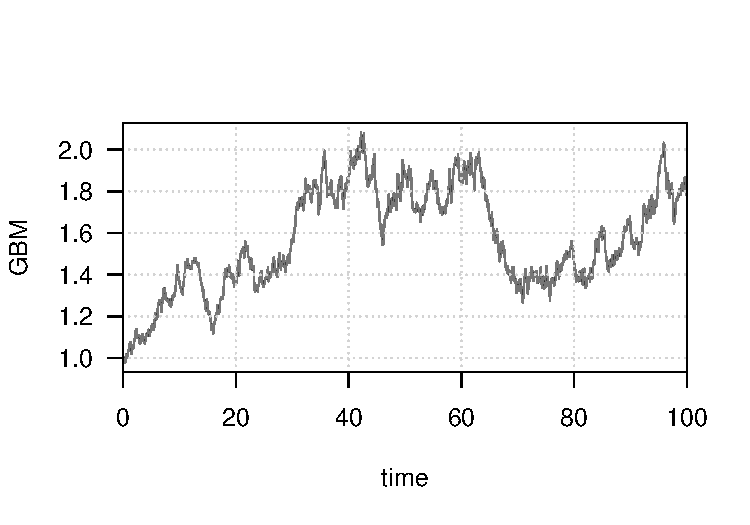
\includegraphics{thesis_files/figure-latex/gbm-1} 
  
  }
  
  \caption{A GBM trajectory path example \label{gbm}}\label{fig:gbm}
  \end{figure}
  \subsection{The model}\label{the-model}
  
  The Black-Scholes model provides analytical solution to the price of a
  European call at time \(t\) and can be described as follows
  {[}1,5,12{]}:
  \begin{align}
  C(S_{t},t)&=N(d_{1})S_{t}-N(d_{2})Ke^{-r(T-t)}\\[10pt]
  d_{1}&={\frac {1}{\sigma {\sqrt {T-t}}}}\left[\ln \left({\frac {S_{t}}{K}}\right)+\left(r+{\frac {\sigma ^{2}}{2}}\right)(T-t)\right]\\[10pt]
  d_{2}&=d_{1}-\sigma {\sqrt {T-t}}
  \end{align}
  \noindent
  Where:
  \begin{itemize}
  \tightlist
  \item
    \(S_{t}\) is the spot price of the underlying asset at time \(t\)
  \item
    \(r\) is the risk free rate (generally an annual
    rate)\footnote{Assumed to be constant. \label{teste}}
  \item
    \(\sigma\) is the volatility of returns of the underlying asset
    \footnote{See footnote 1.}
  \item
    \(N(\cdot )\) is the cumulative distribution function of the standard
    Gaussian distribution
  \item
    \(K\) is the strike price
  \item
    \(T-t\) is the time to maturity
  \end{itemize}
  \noindent
  Also, the stock price path is a Geometric Brownian Motion as previously
  stated, and is under the risk-neutral measure with the following
  dynamics {[}5,18{]}:
  \begin{align}
  dS_{t} = (r-q)S_td_t+\sigma S_t dW_t
  \end{align}
  \noindent
  Where \(dW_t\) is a Wiener process {[}1,18{]}, \(r\) is the risk free
  rate and \(q\) is the dividend
  yield\footnote{$r$ and $q$ are assumed to be constant.} and \(t\)
  denotes the current point in time.
  
  \subsection{Limitations}\label{limitations}
  
  Although the Black-Scholes is very popular and the \emph{de facto}
  standard in the market there are implications to the B-S model
  assumptions that affect the results and that are unrealistic. The main
  assumption that does not hold up is the deterministic (constant)
  volatility, that can more accurately be described as a stochastic
  process since we observe that small moves usually are followed by small
  moves and large moves by large moves. {[}5,12{]}
  
  Other assumptions that are critical to the B-S model and are not always
  observed in practice refer to the asset's continuity through time (no
  jumps), being allowed to perform continuous hedge without transactions
  costs and normal (Gaussian) returns.
  
  Most models focus on the volatility problem because transaction costs
  often translate to rises in volatility and fat-tails (abnormal) returns
  can be simulated by stochastic volatility and market or volatility
  jumps.
  
  \section{Stochastic Volatility
  models}\label{stochastic-volatility-models}
  
  Introducing stochastic volatility to models brings complexity, but
  enables modeling some features observed in reality that are crucial,
  like the randomic market volatility effects, skewness (market returns
  are more realistically modeled) and volatility smile\footnote{The name
    derives from the concave shape of the graph, which resembles a smile.}
  (see Figure \ref{fig:smile}). This kind of model is applied highly
  succesfully in foreign exchange and credit markets.
  
  \BeginKnitrBlock{definition}[Volatility Smile]
  
  \protect\hypertarget{def:unnamed-chunk-4}{}{\label{def:unnamed-chunk-4}
  \iffalse (Volatility Smile) \fi{} }Volatility smiles are implied
  volatility patterns that arise in pricing financial options. In
  particular for a given expiration, options whose strike price differs
  substantially from the underlying asset's price command higher prices
  (and thus implied volatilities) than what is suggested by standard
  option pricing models. These options are said to be either deep
  in-the-money or out-of-the-money.
  
  \EndKnitrBlock{definition}
  
  Furthermore, stochastic volatility models use statistical methods as
  foundations to price and forecast options' behaviors and the
  underlying's security volatility is arbitrary. The Heston, the \(3/2\)
  and other models, like the GARCH\footnote{generalized autoregressive
    conditional heteroscedasticity.} and SABR,\footnote{stochastic alpha,
    beta, rho.} are considered standard smile models.
  \begin{figure}
  
  {\centering 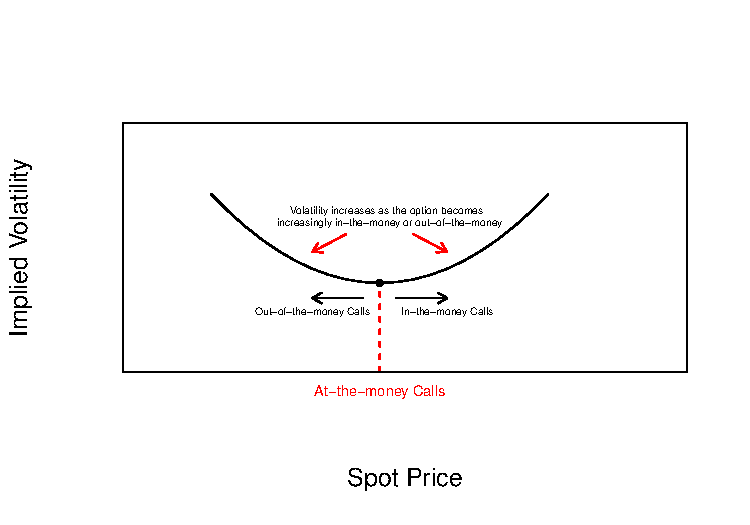
\includegraphics{thesis_files/figure-latex/smile-1} 
  
  }
  
  \caption{Volatility Smile \label{smile}}\label{fig:smile}
  \end{figure}
  \subsection{Cox-Ingersoll-Ross model}\label{cir}
  
  The Cox-Ingersoll-Ross (CIR) model is a well-known short-rate model that
  describes the interest rate movements driven by one source of market
  risk. The dynamics are described as follows{[}19,20{]}:
  \begin{align}
  \label{eq:cir}
  dr_t &= k(\theta - r_t)dt + \sigma \sqrt{r_t} dB_t
  \end{align}
  \noindent
  Where, \(r_t\) is the short rate interest described by parameters
  \(\kappa\) the speed of mean reversion, \(\theta\) the long-run mean
  variance and \(\sigma\) the volatility of the variance process.
  
  This model has been widely used to describe the dynamics of the short
  rate interest because it has some fundamental features like intuitive
  parametrization, nonnegativity and pricing formulas. Besides, it takes
  account of anticipations, risk aversion, investment alternatives and
  preferences about consumption timing and allows for detailed predictions
  about how changes in a wide range of underlying variables affect the
  term structure{[}19{]}. Furthermore, this equation constitutes one of
  the two Heston model equations with the volatility taking the short rate
  interest place.
  
  \subsection{Heston Model}\label{hes1}
  
  Heston model was introduced in 1993 by Steven Heston to solve the
  deterministic volatility problems. It was designed to analize bond and
  currency options and it introduced the following equations, which
  represent the dynamics of the stock price and the variance processes
  under the risk-neutral measure {[}20,21{]}:
  \begin{align}
  \label{eq:heston}
  dS_t &= \mu S_t dt + \sqrt{V_t} S_t dW^*_t \\
  dV_t &=  \kappa (\theta - V_t)dt + \sigma \sqrt{V_t} dB_t
  \label{eq:hesvar}
  \end{align}
  The second equation, as described in Section \ref{cir}, is the CIR model
  equation. The first equation states the asset price process. \(\mu\) is
  the asset's rate of return, \(dW_{t,1}\) and \(dW_{t,2}\) are two
  correlated wiener processes with correlation coefficient of \(\rho\).
  
  \subsection{Other Models}\label{other-models}
  
  \subsubsection{Ornstein-Uhlenbeck}\label{ornstein-uhlenbeck}
  
  The Ornstein-Uhlenbeck is the earliest recorded SDE. Named after Leonard
  Ornstein and George Eugene Uhlenbeck, it is a stochastic process that
  describes the acceleration of a pollen particle in a liquid subject to
  bombardments by molecules {[}3{]}. As we can observe in equation
  \eqref{eq:oueq}, \(x_t\) represents the one dimension velocity of the
  particle, thus \(dx_t\) is the \emph{change} in velocity, in other
  words, its acceleration. The \(- \theta x_t\) component slows down the
  acceleration and is to be understood as frictional force. Besides, we
  add a noise \(W_t\) with intensity \(\sigma\) that models the random
  bombardment by the molecules.
  \begin{align} 
  \label{eq:oueq}
  &d x_t = - \theta x_t dt + \sigma d W_t
  \end{align}
  With \(\theta\) and \(\sigma\) being positive constants. Expressing in
  terms of \(x_t\) we get:
  \begin{align}
  x_t = e^{-\theta t} \times \left[ x_0  + \sigma \int_{t=0}^{T} e^{\theta t} d W_s \right] \,.
  \end{align}
  \subsubsection{Langevin}\label{langevin}
  
  The Langevin equation describes a system that consists of the molecular
  bombardment of a speck of dust on a water surface. We know that the
  intensity of the bombardement does not depend on the state variables
  {[}22,23{]}.
  \begin{align}
  m \frac{dv}{dt} = -\zeta v + \delta F (t) 
  \end{align}
  \(m\) is the mass of the particle, \(v\) it's velocity, \(-\zeta v\) is
  the frictional force, which is proportional to the velocity, and
  \(\delta F (t)\) is a \emph{fluctuating} force (random) to the
  frictional force.
  
  \section{Numerical Methods}\label{numerical-methods}
  
  Numerical methods are tools that are often applied to solve stochastic
  differential equations because most of these do not have explicit
  solution. This means that we are not able to solve these equations using
  symbolic computation. Although we are unable to find an analitical
  solution, when facing real problems, the approximation given by a
  numerical method is often sufficient. Alongside the analytical issue,
  the need to calculate the SDE's trajectory through time is the main
  reason why studying numerical methods is so important. An implementation
  of a numerical method is called a numerical algorithm.
  
  We will simulate sample paths of time discrete approximations
  implemented in the R programming language {[}2{]} that we base on a
  finite discretization of a time interval \([t_0, T]\). We shall generate
  approximate values of the sample path for each step contained in the
  discretized interval {[}22{]}.
  
  In the fixed step methods, the distance between two contiguous points is
  the distance
  \(d_i = t_i - t_{i-1} = \frac{T-t_0}{N} \;\;\; \forall i \mid 1 \leq i \leq N \in \mathbb{N}\).
  \(N\) being the time interval partition number.
  
  According to Kloeden {[}22{]}, in the stochastic realm, simulated sample
  paths can be statistically analysed to find how good an approximation is
  compared to an exact solution. Moreover, the computational costs such as
  time and memory increases polynomially with the problem's dimension,
  which is good, and it is possible to apply variance reduction methods
  that allow a considerable decrease in the required sample size.
  
  \subsection{Convergence}\label{convergence}
  
  As soon as we talk about numerical methods we are required to approach
  the topic of approximations and how to handle them. Methods efficiency
  receive the name of \emph{convergence order}. In the SDE domain there
  are two main methods of convergency, that are classified according to
  their criteria. Firstly, we present the \emph{strong order of
  convergence}. A method is said to have strong convergence \(\delta\) to
  \(Y\) if a time discretized \(Y_{\delta}\) of a continous-time process
  \(Y\), with \(\delta\) being the maximum time increment of the
  discretization, and for any fixed time horizon \(T\) holds true that
  {[}16{]}:
  \begin{align*}
  \mathbb{E} \mid Y_{\delta}(T) - Y(T) \mid \leq C \delta^{\gamma}, \,\,\, \forall \delta < \delta_0
  \end{align*}
  with \(\delta_0 > 0\) and \(\mathcal{C}\) a constant not depending on
  \(\delta\). Strong convergence addresses the problem of solutions'
  trajectories. For specific conditions, the Euler method has strong
  convergence order \(\gamma = \frac{1}{2}\). Furthermore, there is the
  \emph{weak order of convergence}. The weak convergence
  \begin{align*}
  \mid  \mathbb{E}p(Y_n) - \mathbb{E}p(Y(\tau)) \mid \leq C \Delta t^{\gamma}
  \end{align*}
  Strong and weak convergence are not mutually exclusive {[}16{]}. That
  means that a method with a given strong order of convergence might have
  a higher weak order of convergence too. This is the case for the Euler
  scheme, with a strong order of convergence of \(1/2\) and a weak order
  of \(1\) (under some conditions). For a more detailed and rigorous
  explanation of convergence we recommend consulting {[}24{]}.
  
  It is worth noting that, altough schemes have a given convergency order,
  it is not unusual that they behave better than their order for some SDEs
  specifications.
  
  \subsection{Discretization}\label{discretization}
  
  We know that convergence is an important feature to a numerical method
  and studies have found not all time discrete possible approximations of
  an SDE converge in a useful sense to the solution process as the step
  size adopted tends toward zero {[}25,26{]}. Moreover, particularly for
  SDEs, some of the more rapidly convergent methods available for ordinary
  differential equations (ODE) do not work, such as higher order
  Runge-Kutta methods.\footnote{The euler method is the simplest
    Runge-Kutta method.}
  
  One of the methods that do work for ODEs and SDEs is the Euler method,
  named after the Swiss mathematician Leonhard Euler. Figure
  \ref{fig:euler} shows an example of an implementation for the Newton's
  cooling law with timestep of 2 seconds compared to its analytical
  solution. This method (\emph{a.k.a.} forward Euler method) is a
  first-order numerical procedure. It is the most basic explicit
  method\footnote{Explicit methods calculate the state of a system at a
    later time from the state of the system at the current time.
    Mathematically we have something like \(Y(t+\Delta t)=F(Y(t))\,\).}
  for numerical integration.
  \begin{figure}
  
  {\centering 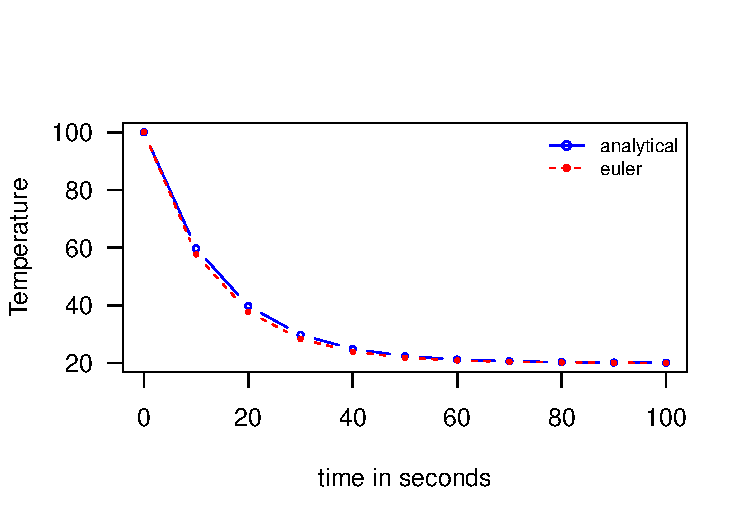
\includegraphics{thesis_files/figure-latex/euler-1} 
  
  }
  
  \caption{Analytical x Euler solutions \label{euler}}\label{fig:euler}
  \end{figure}
  The method is first-order, as stated above, this means that the error in
  each step is a proportion of the square of the step size. Also, the
  global error at a given time is a function of the step size. We proceed
  to apply the Euler method to SDEs. Consider the equation:
  \begin{align}
  dS_t &= \mu(S_t,t) dt + \sigma(S_t,t) dW_t
  \end{align}
  \(dW_t\) is the Brownian motion, \(\mu\) and \(\sigma\) are functions
  depending on \(S_t\) and \(t\), over an interval \([0,T]\), and we want
  to discretize it as \(0 = t_1 < t2 < \cdots < t_m = T\) with increments
  equally spaced \(d_t\).
  
  Integrating it from \(t\) to \(dt\) we have the starting point for our
  (and any) discretization scheme:
  \begin{align}
  \label{eq:disc1}
  S_{t+dt} &= S_t + \int_{t}^{dt}{\mu(S_u,u)}du + \int_{t}^{dt}{\sigma(S_u,u)} dW_u
  \end{align}
  To use the Euler discretization is the equivalent of approximating
  integrals using the left-point rule as in Figure
  \ref{graph_euler}\footnote{See Kiusalaas {[}27{]}}, we then have:
  \begin{align*}
   \int_{t}^{t+dt}{\mu(S_u,u)} dW_u &\approx \mu(S_t,t) \int_{t}^{t+dt}dW_u\\
  &= \mu(S_t,t) (W_{t+dt} - W_t)  \\
   \int_{t}^{t+dt}{\sigma(S_u,u)} dW_u &\approx \sigma(S_t,t) \int_{t}^{t+dt}dW_u\\
  &= \sigma(S_t,t) (W_{t+dt} - W_t)  \\
  &= \sigma(S_t,t) \sqrt{dt} Z
  \end{align*}
  \(W_{t+dt}-W_t\) and \(\sqrt{dt}Z\) have identical distribution, \(Z\)
  being a standard gaussian variable. The Euler discretization of equation
  \eqref{eq:disc1} is then:
  \begin{align}
  \label{eq:disc2}
  S_{t+dt} &= S_t + \mu(S_t,t)dt + \sigma(S_t,t)\sqrt{dt}Z
  \end{align}
  \begin{figure}
  \begin{center}
      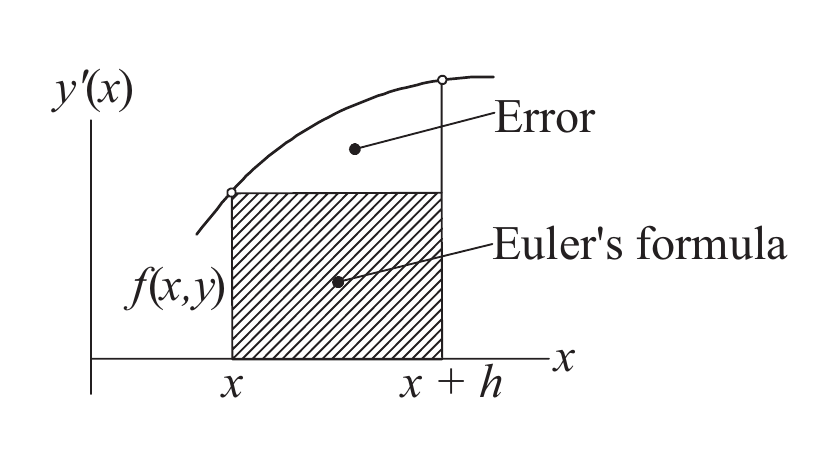
\includegraphics[width=100mm]{figure/euler_screen.png}
      \caption{Graphical representation of Euler’s formula}\label{graph_euler}
      \caption*{\scriptsize{Source: Numerical methods in Engineering with Python 3.}}
  \end{center}
  \end{figure}
  \subsubsection{Euler method - Heston
  model}\label{euler-method---heston-model}
  
  We now proceed to apply the method to our model of interest. We retake
  the equations \eqref{eq:heston} and \eqref{eq:hesvar}. We begin showing how
  to discretize the latter {[}16,24{]}:
  \begin{align}
  \label{eq:hesvareuler}
  V_{t+dt} = V_t+ \int_{t}^{t+dt}{\kappa (\theta - V_u) du} + \int_{t}^{t+dt}{\sigma \sqrt{V_u} dB_u}
  \end{align}
  Which discretized turns out as:
  \begin{align*}
   \int_{t}^{t+dt}{\kappa (\theta - V_u)} du &\approx \kappa (\theta - V_t) dt\\
   \int_{t}^{t+dt}{\sigma \sqrt{V_u}} dB_t &\approx \sigma \sqrt{V_t} (W_{t+dt}-W_t)\\
  &= \sigma \sqrt{V_t dt} Z_v
  \end{align*}
  And leaves us with:
  \begin{align}
  V_{t+dt} = V_t + \kappa (\theta - V_t) dt + \sigma \sqrt{V_t dt} Z_v
  \end{align}
  \(Z_v\) is a standard normal variable. To avoid problems with negative
  values in \(\sqrt{V_t}\) we apply the \emph{full truncation} scheme,
  which substitutes \(V_t\) with \(V_t^+ = max(0, V_t)\).\footnote{Another
    possible scheme (not used in this work) is the \emph{reflection}
    scheme where we replace \(V_t\) with \(\mid V_t \mid\)}
  
  For the \(S_t\) SDE we proceed similarly:
  \begin{align}
  \label{eq:heseuler}
  S_{t+dt} = S_t+ \mu \int_{t}^{t+dt}{ S_u du} + \int_{t}^{t+dt}{\sqrt{V_u} S_u dW_u}
  \end{align}
  Discretizing we have:
  \begin{align*}
   \int_{t}^{t+dt}{S_u} du &\approx S_t dt\\
   \int_{t}^{t+dt}{\sqrt{V_u} S_u} dW_u &\approx \sqrt{V_t} S_t (W_{t+dt}-W_t)\\
  &= \sqrt{V_t dt} S_t Z_s
  \end{align*}
  \(Z_s\) is a standard normal variable with correlation \(\rho\) with
  \(Z_v\). We have:
  \begin{align}
  S_{t+dt} = S_t + \mu S_t dt + \sqrt{V_t dt} S_t Z_s
  \end{align}
  \subsection{Stability}\label{stability}
  
  Most differential equations, deterministic or stochastic, cannot be
  solved explicitly {[}22{]}. Hence, stability studies begin with
  computers and is associated with numerical methods and approximations.
  Convergent methods were resulting in bigger errors than what was
  expected that could not be only due to discretization error. Eventually,
  scientists discovered that this unexpected problem was caused by
  accumulation of successive truncation errors. Figure \ref{fig:stab}
  retakes the cooling example previously approached to show instability
  due to an increase in size of the timestep and extending to \(600\)
  seconds. The top plot, with a step of \(25\) still converges to the real
  solution, but we already observe an odd behaviour since the numerical
  method doesn't follow the analytical solution, but instead revolver
  around it until convergence. The bottom plot, presents a small increase
  in the step \(h = 29\), and this small increment is enough results in
  numbers completely off target.
  \begin{figure}
  
  {\centering 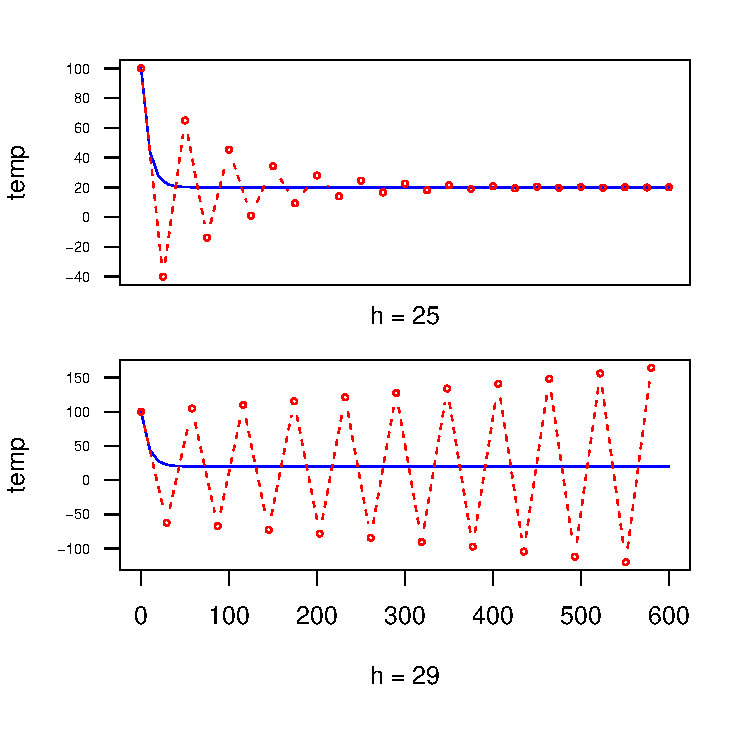
\includegraphics{thesis_files/figure-latex/stab-1} 
  
  }
  
  \caption{Euler's stability whith different timesteps \label{stab}}\label{fig:stab}
  \end{figure}
  We know that binary machines like computers are not able to represent
  all the real numbers, but only a subset of them. Thus, solving these
  errors is not straightforward since it's not possible to eliminate
  \emph{all} truncation error when using a computer and dealing with
  numerical solutions. When faced to an incorrect (not acceptable)
  solution, we have to evaluate and distinguish between two distinct
  situations:
  \begin{itemize}
    \item [i] Rounding errors are considerably amplified by the algorithm. This situation is called numerical instability.
    \item [ii] Small perturbations of data generate large changes in the solution. This is termed an ill-conditioned (or sensitive) problem.
  \end{itemize}
  Examples of these two classes of problem can be found in {[}21{]}.
  
  Stiff equations appear very often in mathematical problems and refer to
  differential equations for which a numerical methods might be unstable
  for not small enough stepsizes {[}28{]}. A differential equation of the
  form \(y' = f(t,y)\), if its exact solution \(y(t)\) includes a term
  that decays exponentially to zero as \(t\) increases, but whose
  derivatives are greater in magnitude than the term itself. In other
  words, if it requires a significant depression of the stepsize to avoid
  stability lost. This is a loose definition but, since we are dealing
  with numerical methods a proper mathematical definition isn't required.
  Tipically, these equations are of the form \(e^{-ct}\), where \(c\) is a
  large positive constant {[}29{]}. A practical example of the stiff
  behavior is the following differential equation {[}30{]}:
  \begin{align*}
  y' = -100y, \,\,\,\,\,\, t > 0, \,\,\,\,\,\, y_0 = 1
  \end{align*}
  Whose exact solution is \(y_t = e^{-100 t}\) and goes to zero as \(t\)
  increases. Applying Euler's method to this equation with \(h=0.1\) we
  stumble in the following equation
  \begin{align*}
  y_{n+1} = y_{n} - 100 h y_{n} = -9y_{n}
  \end{align*}
  which is wrong, since it yields an exponencially growing solution
  \(y_n = (-9)^n\). On the other hand, if our timestep is smaller
  \(h = 10^{-3}\), our solution using Euler's method becomes
  \(y_n = (0.9)^n\). This solution leads to an accurate behavior regarding
  the exact solution, it rapidily decays to zero.
  
  Sometimes, it is interesting to rank differential equations that are
  more or less stiff. Thus, people compute the quotient of the largest and
  the smallest eigenvalues of a linear system. They call it the equations'
  \textit{stiffness ratio} and, usually the bigger the stiffness ratio,
  the more likely is to be stiff {[}28{]}.
  
  \subsubsection{Stability Domain}\label{stability-domain}
  
  Let's take the equation:
  \begin{align}
  y' = \lambda y,  \,\,\,\,\,\, t \geq 0, \,\,\,\,\,\,\,\,\,\,\,\,\,\, y_0 = 1
  \end{align}
  where \(\lambda \in \mathbb{C}\) or in other terms
  \(\lambda = \lambda_r + i \lambda_i\) and whose solution is
  \(y+t = e^{\lambda t}\). We can rewrite this equation as a system:
  \begin{align}
  \frac{d}{dt} \begin{bmatrix} y^1 \\ y^2 \end{bmatrix} = 
  \begin{pmatrix} 
  \lambda_r & - \lambda_i \\
  \lambda_i & - \lambda_r 
  \end{pmatrix}
  \begin{bmatrix} y^1 \\ y^2 \end{bmatrix}
  \end{align}
  The \(\lim_{t \to \infty} y_t = 0\) if and only if
  \(\mathbb{R} \lambda < 0\). The \emph{linear stability domain}
  \(\mathcal{D}\) is defined as the set of all numbers
  \(\Delta \lambda \in mathbb{C}\) such that
  \(\lim_{n \to \infty y+n = 0}\), with \(\Delta > 0\) being the stepsize.
  Or, as stated in Kloeden {[}22{]}, the suitable values of the stepsize
  are expressed in terms of \emph{region of absolute stability},
  consisting of the complex numbers \(\lambda \Delta\) for which an error
  in \(y_0\) at \(t_0\) will not grow in subsequent iterations of the
  method.
  
  Without entering all the details, for these we recommend {[}22,28,30{]},
  the euler's stability domain is:
  \begin{align*}
  \mathcal{D}_{Euler} = z \in \mathbb{C} : \mid 1 + z \mid < 1
  \end{align*}
  which represents the interior of a complex disc of unit radius and
  centre \(z = -1\) as can be seen in Figure \ref{stab2}, on the left. The
  right side of the Figure \ref{stab2} shows the stability region called
  A-stability.\footnote{Mathematically:
    \(\mathcal{D} \subseteq \left\{ z \in \mathbb{C} : \mathbb{R} z < 0 \right\}\).}
  If a method is A-stable, the stepsize \(\Delta\) is only constraint by
  accuracy.
  \begin{figure}
  
  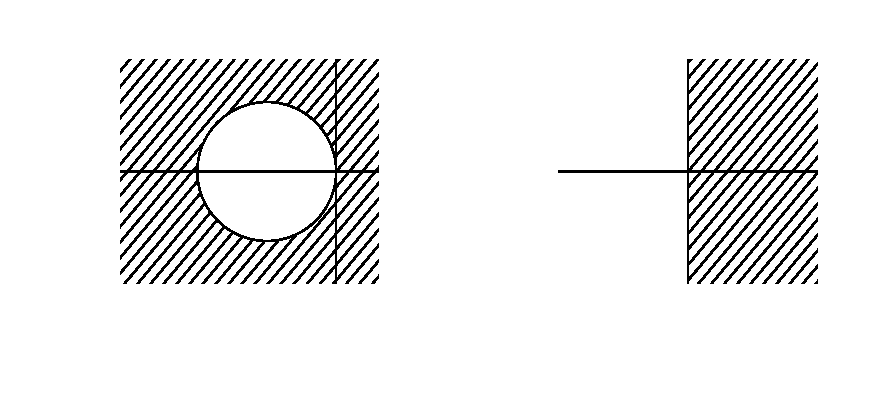
\includegraphics{thesis_files/figure-latex/stab2-1} \hfill{}
  
  \caption{Stability domains \label{stab2}}\label{fig:stab2}
  \end{figure}
  Thereby, we claim that stability method study is an important topic,
  since it enables achieving solutions that are good to stiff equations
  without having to overly reduce our timesteps which can be very
  computationally costly.
  
  \chapter{The Heston Model Implementation}\label{implement}
  
  In section \ref{hes1} we presented Heston's SDE system in one of its
  structures. Another common way {[}31--33{]} to write down the system is
  using the property presented in subsection \ref{corr} as in equation
  \eqref{eq:heston2}.
  \begin{align}
  \label{eq:heston2}
  \begin{split}
  dS_t &= \mu S_t dt + \rho \sqrt{V_t} dB_t + \sqrt{1 - \rho^2} \sqrt{V_t} S_t dW_t \\
  dV_t &= k(\theta - V_t)dt + \sigma \sqrt{V_t} dB_t 
  \end{split}
  \end{align}
  \section{Characteristic Function}\label{characteristic-function}
  
  The Heston model characteristic function is firstly presented in the
  1993 Steven Heston's paper {[}20{]} and is described below {[}34{]}:
  \begin{align}
  f(S_t, V_t, t) = e^{A(T-t)+B(T-t)S_t + C(T-t)V_t + i \phi S_t}
  \end{align}
  If we let \(\tau = T-t\), then the explicit form of the Heston
  characteristic function is:
  \begin{align*}
  f(i \phi) &= e^{A(\tau)+B(\tau)S_t + C(\tau)V_t + i \phi S_t} \\
  A(\tau) &= r i \phi \tau + \frac{\kappa \theta}{\sigma^2} \left[ - (\rho \sigma i \phi - \kappa - M) \tau - 2 \ln\left(\frac{1-N e^{M \tau}}{1-N}\right) \right] \\
  B(\tau) &= 0 \\
  C(\tau) &= \frac{(e^{M \tau}-1)(\rho \sigma i \phi - \kappa - M)}{\sigma^2 (1-N e^{M \tau})} \\
  \text{Where:} & \\
  M &= \sqrt{(\rho \sigma i \phi - \kappa)^2 + \sigma^2 (i \phi + \phi^2)} \\
  N &= \frac{\rho \sigma i \phi - \kappa - M}{\rho \sigma i \phi - \kappa + M} \\
  \end{align*}
  This function is the driving force behind the following formula, that
  calculates the fair value of a European call option at time \(t\), given
  a strike price \(K\), that expires at time \(T\) {[}34{]}:
  \begin{align} 
  \label{eq:cfheston}
  \begin{split}
  C = & \frac{1}{2} S(t) + \frac{e^{-r(T-t)}}{\pi}\int_{0}^{\infty}{\Re \left[ \frac{K^{-i \phi} f(i \phi + 1)}{i \phi} \right] d\phi} \\
  & -Ke^{-r(T-t)}\left( \frac{1}{2} + \frac{1}{\pi} \int_{0}^{\infty}{\Re \left[ \frac{K^{-i \phi} f(i \phi)}{i \phi} \right]}  d\phi \right)
  \end{split}
  \end{align}
  \section{Euler Scheme}\label{euler-scheme}
  
  Given the fact that the underlying asset is temporal dependent upon the
  solution of the SDE's volatility, we simulate the volatility's path
  before the asset's. If the Black-Scholes model enabled using Ito's Lemma
  directly for solving \(S_t\), this equation system requires numerical
  methods. We present here the Euler Scheme - Full Truncation algorithm
  (and compare to other similar schemes) {[}31{]} along with some insights
  on how it was implemented in R. The Euler discretization brings
  approximation paths to stock prices and variance processes. If we set
  \(t_0 = 0 < t_1 < \dots < t_M = T\) as partitions of a time interval of
  \(M\) equal segments of length \(\delta t\), we have the following
  discretization for the stock price:
  \begin{align}
  S_{t+1} = S_t + rS_t + \sqrt{V_t} S_t Z_s
  \end{align}
  \noindent
  And for the variance process:
  \begin{align}
  V_{t+1} = f_1(V_{t}) + \kappa (\theta - f_2(V_{t})) + \sigma \sqrt{f_3(V_{t})} Z_v 
  \end{align}
  \noindent
  \(Z_s\) being a standard normal random variable, i.e. \(N\sim(0,1)\), we
  set \(Z_t\) and \(Z_v\) as two independent standard normal random
  variables and \(Z_s\) and \(Z_v\) having correlation \(\rho\). This
  means we can write \(Z_s = \rho Z_v + \sqrt{1-\rho^2} Z_t\).
  
  The immediate observable problem in the proposed discretization scheme
  is that \(V\) can become negative with non-zero probability making the
  computation of \(\sqrt{V_t}\) impossible {[}32{]}. There are several
  proposed fixes that can be used as you can see below:
  \begin{table}[ht]
  \centering
  \begin{tabular}{cccc}
    \hline 
  Scheme & $f_1(V_{t})$ & $f_2(V_{t})$ & $f_3(V_{t})$ \\ 
    \hline 
  Reflection & $\mid V \mid$ & $\mid V \mid$ & $\mid V \mid$ \\ 
    Partial Truncation & $V$ & $V$ & $V^+$ \\ 
    Full Truncation & $V$ & $V^+$ & $V^+$ \\ 
     \hline 
  \end{tabular}
  \caption{Truncation schemes} 
  \label{box}
  \end{table}
  Where \(V^+ = \max(V,0)\) and \(\mid V \mid\) is the absolute value of
  \(V\).
  
  We chose to fix our discretization using the Full-Truncation (FT) scheme
  and thus, rewrite the equations as follows:
  \begin{align}
  \label{eq:st1}
  S_{t+1} &= S_t + rS_t + \sqrt{V_{t}^{+}} S_t Z_s \\
  \label{eq:vt1}
  V_{t+1} &= V_t + \kappa (\theta - V_{t}^{+}) + \sigma \sqrt{V_{t}^{+}} Z_v 
  \end{align}
  Our R implementation follows the euler's scheme with hardly any
  modifications. It draws two Gaussian random variables (\(Z_v\) and
  \(Z_t\)) using the function \emph{rnorm} to create \(Z_s\) with
  correlation \(\rho\) with \(Z_v\).
  \begin{Shaded}
  \begin{Highlighting}[]
  \NormalTok{  Zv <-}\StringTok{ }\NormalTok{stats}\OperatorTok{::}\KeywordTok{rnorm}\NormalTok{(N)}
  \NormalTok{  Zt <-}\StringTok{ }\NormalTok{stats}\OperatorTok{::}\KeywordTok{rnorm}\NormalTok{(N)}
  \NormalTok{  Zs <-}\StringTok{ }\NormalTok{rho }\OperatorTok{*}\StringTok{ }\NormalTok{Zv }\OperatorTok{+}\StringTok{ }\NormalTok{(}\KeywordTok{sqrt}\NormalTok{(}\DecValTok{1} \OperatorTok{-}\StringTok{ }\NormalTok{(rho}\OperatorTok{^}\DecValTok{2}\NormalTok{)) }\OperatorTok{*}\StringTok{ }\NormalTok{Zt)}
  \end{Highlighting}
  \end{Shaded}
  And use it to compute \(S\) and \(V\) as in the code snippet bellow. The
  two modifications we apply are previously computing the square roots of
  the stepsize \emph{dt} and the \emph{aux} variable as to improve speed.
  The \emph{aux} variable is an help variable created to impose positivity
  to \(V\) as we are operating the full-truncation euler scheme.
  \begin{Shaded}
  \begin{Highlighting}[]
  \NormalTok{  S <-}\StringTok{ }\NormalTok{S }\OperatorTok{*}\StringTok{ }\NormalTok{(}\DecValTok{1} \OperatorTok{+}\StringTok{ }\NormalTok{r }\OperatorTok{*}\StringTok{ }\NormalTok{dt }\OperatorTok{+}\StringTok{ }\NormalTok{sqrt_aux }\OperatorTok{*}\StringTok{ }\NormalTok{Zs }\OperatorTok{*}\StringTok{ }\NormalTok{sqrt_dt)}
  \NormalTok{  v <-}\StringTok{ }\NormalTok{v }\OperatorTok{+}\StringTok{ }\NormalTok{k }\OperatorTok{*}\StringTok{ }\NormalTok{dt }\OperatorTok{*}\StringTok{ }\NormalTok{(theta }\OperatorTok{-}\StringTok{ }\NormalTok{aux) }\OperatorTok{+}\StringTok{ }
  \StringTok{                     }\NormalTok{sigma }\OperatorTok{*}\StringTok{ }\NormalTok{sqrt_aux }\OperatorTok{*}\StringTok{ }\NormalTok{Zv }\OperatorTok{*}\StringTok{ }\NormalTok{sqrt_dt}
  \end{Highlighting}
  \end{Shaded}
  We could have used the \emph{pmax} function in R, but this function is
  slow, therefore we opted to create the \emph{aux} variable and impose
  positive values using the following R syntax:
  \begin{Shaded}
  \begin{Highlighting}[]
  \NormalTok{  aux <-}\StringTok{ }\NormalTok{v}
  \NormalTok{  aux[v }\OperatorTok{<}\StringTok{ }\DecValTok{0}\NormalTok{] <-}\StringTok{ }\DecValTok{0}
  \end{Highlighting}
  \end{Shaded}
  Depending on the reader's R fluency, other parts of the scheme might
  present a challenge, and that is why a version of the function is fully
  presented in appendix \ref{eulerapp}.
  
  \section{Kahl-Jackel}\label{kahl-jackel}
  
  Kahl-Jackel propose a discretization method they refer to as the ``IJK''
  method {[}32,33{]} that coupled with the implicit Milstein scheme for
  the variance lands the system of equations \eqref{eq:kj1} and
  \eqref{eq:kj2}. It is possible to verify that this discretization always
  results in positive paths for \(V\) if \(4 \kappa \theta > \sigma^2\).
  Unfortunately, this inequality is rarely satisfied when we plug real
  market data to calibrate the parameters. This means we must have a
  defined strategy for when the inequality doesn't hold. We use the scheme
  proposed in Andersen {[}32{]}, where a truncation similar to the Euler's
  is applied. Whenever our volatility \(V_t\) drops below zero we use
  \eqref{eq:vt1}, and implement \(\hat{V}(t+\Delta)^{+}\) and
  \(\hat{V}(t)^{+}\) instead of \(\hat{V}(t+\Delta)\) and \(\hat{V}(t)\)
  of equation \eqref{eq:kj1}. The code guidance to this method can be found
  in appendix \ref{kjimp}.
  \begin{small}
  \begin{align}
  \label{eq:kj1}
  \ln \hat{S}(t + \Delta) &= \ln \hat{S}(t) - \frac{\Delta}{4}\left( \hat{V}(t+\Delta) + \hat{V}(t) \right) + \rho \sqrt{\hat{V}(t)}Z_v\sqrt{\Delta} \\ \nonumber
  &+ \frac{1}{2} \left( \sqrt{\hat{V}(t+\Delta)} + \sqrt{\hat{V}(t)} \right) \left( Z_S \sqrt{\Delta} - \rho Z_V \sqrt{\Delta}\right) + \frac{1}{4} \sigma \rho \Delta \left( Z_{V}^{2} - 1 \right) \\
  \label{eq:kj2}
  \hat{V}(t+\Delta) &= \frac{\hat{V}(t) + \kappa \theta \Delta + \sigma \sqrt{\hat{V}(t)}Z_V \sqrt{\Delta}+ \frac{1}{4}\sigma^2 \Delta \left(Z_V^2-1 \right)}{1+ \kappa \Delta}
  \end{align}
  \end{small}
  \section{Exact Algorithm}\label{exact-algorithm}
  
  In 2006, Broadie-Kaya {[}31{]} propose a method that has a faster
  convergence rate, \(\mathcal{O} \left( s^{-1/2} \right)\) than some of
  the more famous schemes, such as Euler's and Milstein's discretizations.
  They build their idea to generate an exact sample from the distribution
  of the terminal stock price based on numerous papers {[}20{]}. The stock
  price and variance are as follows:
  \begin{align} \label{eq:ea1}
  S_t = S_0 \, exp \left[ \mu t - \frac{1}{2} \int_{0}^{t}{V_s ds} + \rho  \int_{0}^{t}{\sqrt{V_s d B_s}} + \sqrt{1 - \rho^2} \int_{0}^{t}{\sqrt{V_s} dW_s}\right]
  \end{align}
  The squared volatility of the variance process is:
  \begin{align} \label{eq:ea2}
  V_t = V_0 + \kappa \theta t - \kappa \int_{0}^{t}{V_s ds} + \sigma \int_{0}^{t}{\sqrt{V_s dB_s}}
  \end{align}
  The algorithm used to generate the model consists in four steps as
  follows:
  \begin{itemize}
  \item [\textit{Step} 1.] Generate a sample of $V_t$ given $V_0$
  \item [\textit{Step} 2.] Generate a sample of $\displaystyle \int_0^t V_sds$ given $V_t$, $V_0$
  \item [\textit{Step} 3.] Compute $displaystyle \int_0^t \sqrt{V_s}dB_s$ given $V_t$, $V_0$ and $\int_0^t V_sds$
  \item [\textit{Step} 4.] Generate a sample from the probability distribution of $S_t$, given $displaystyle \int_0^t \sqrt{V_s}dB_s$ and $displaystyle \int_0^t V_sds$
  \end{itemize}
  \subsection{\texorpdfstring{Generate a sample of \(V_t\) given
  \(V_0\)}{Generate a sample of V\_t given V\_0}}\label{generate-a-sample-of-v_t-given-v_0}
  
  The distribution of \(V_t\) given \(V_0\) for \(0 < t\) is a non-central
  chi-squared distribution {[}19,38{]}:
  
  \[V_t = \frac{\sigma^2 (1-e^{- \kappa t})}{4 \kappa} \chi_{\delta}^{2} \left( \frac{4 \kappa e^{- \kappa t}}{\sigma^2 (1- e^{- \kappa t})} \times V_0\right)\]
  
  where \(\delta = \frac{4 \theta \kappa}{\sigma^2}\) and
  \(\chi_{\delta}^{2}(\lambda)\) denotes a non-central chi-squared random
  variable with \(\delta\) degrees of freedom and \(\lambda\) as its
  non-centrality parameter.
  
  Broadie and Kaya {[}31{]} sample generating Poisson and gamma
  distributions as in Johnson et al. {[}39{]}. We used the built-in
  function in R \emph{rchisq}, which uses this exact method for sampling,
  see chunk below.
  \begin{Shaded}
  \begin{Highlighting}[]
  \NormalTok{  d1 <-}\StringTok{ }\NormalTok{(}\DecValTok{4} \OperatorTok{*}\StringTok{ }\NormalTok{k }\OperatorTok{*}\StringTok{ }\NormalTok{theta)}\OperatorTok{/}\NormalTok{(sigma)}\OperatorTok{^}\DecValTok{2}
  \NormalTok{  c0 <-}\StringTok{ }\NormalTok{(sigma}\OperatorTok{^}\DecValTok{2} \OperatorTok{*}\StringTok{ }\NormalTok{(}\DecValTok{1} \OperatorTok{-}\StringTok{ }\KeywordTok{exp}\NormalTok{(}\OperatorTok{-}\NormalTok{k}\OperatorTok{*}\NormalTok{tau)))}\OperatorTok{/}\NormalTok{(}\DecValTok{4}\OperatorTok{*}\NormalTok{k)}
  \NormalTok{  dt <-}\StringTok{ }\NormalTok{(tau}\OperatorTok{-}\NormalTok{t)}
  
    \CommentTok{# sampling V}
  \NormalTok{  lambda <-}\StringTok{ }\NormalTok{(}\DecValTok{4}\OperatorTok{*}\NormalTok{k}\OperatorTok{*}\KeywordTok{exp}\NormalTok{(}\OperatorTok{-}\NormalTok{k}\OperatorTok{*}\NormalTok{dt)}\OperatorTok{*}\NormalTok{v)}\OperatorTok{/}\NormalTok{(sigma}\OperatorTok{^}\DecValTok{2} \OperatorTok{*}\StringTok{ }\NormalTok{(}\DecValTok{1}\OperatorTok{-}\KeywordTok{exp}\NormalTok{(}\OperatorTok{-}\NormalTok{k}\OperatorTok{*}\NormalTok{dt)))}
  \NormalTok{  vt <-}\StringTok{ }\NormalTok{c0 }\OperatorTok{*}\StringTok{ }\NormalTok{stats}\OperatorTok{::}\KeywordTok{rchisq}\NormalTok{(}\DataTypeTok{n =} \DecValTok{1}\NormalTok{, }\DataTypeTok{df =}\NormalTok{ d1, }\DataTypeTok{ncp =}\NormalTok{ lambda)}
  \end{Highlighting}
  \end{Shaded}
  \subsection{\texorpdfstring{Generate a sample of \(\int_0^t V_sds\)
  given \(V_t\),
  \(V_0\)}{Generate a sample of \textbackslash{}int\_0\^{}t V\_sds given V\_t, V\_0}}\label{generate-a-sample-of-int_0t-v_sds-given-v_t-v_0}
  
  After generating \(V_t\), we follow the instructions in {[}31,39{]}. We
  use the characteristic function \eqref{eq:phi} to compute the probability
  density function \(F(x)\).
  \begin{align} \label{eq:phi}
  \begin{split}
  \Phi(a) &= \mathbb{E}\left[ exp \left( ia \int_{0}^{t}{V_s ds} \mid V_0,V_t \right)  \right] \\[10pt]
  &= \frac{\gamma(a)e^{(-1/2)(\gamma(a)- \kappa) t} (1 - e^{- \kappa t})}{\kappa (1 - e^{- \gamma(a) t})} \\[10pt]
  &\times exp \left\{\frac{V_0 + V_t}{\sigma^2} \left[ \frac{\kappa (1 + e^{- \kappa t})}{1 - e^{- \kappa t}} - \frac{\gamma(a) (1 + e^{- \gamma(a) t})}{1 - e^{- \gamma(a) t}} \right] \right\} \\[10pt]
  &\times \frac{I_{0.5\delta - 1} \left[ \sqrt{V_0 V_t} \frac{4 \gamma(a) e^{-0.5 \gamma(a) t}}{\sigma^2 (1 - e^{- \gamma(a) t})} \right]}{I_{0.5\delta - 1}  \left[ \sqrt{V_0 V_t} \frac{4 \kappa e^{-0.5 \kappa t}}{\sigma^2 (1 - e^{- \kappa t})} \right]}
  \end{split}
  \end{align}
  where \(\gamma(a) = \sqrt{\kappa^2 - 2 \sigma^2 i a}\), \(\delta\) was
  previously defined and \(I_v(x)\) is the modified Bessel function of the
  first kind.\footnote{\textit{See Appendix  \\ref{bessel} for more information.}}
  There are no mysteries implementing the characteristic function as you
  can observe in the chunk below. Although R has a built-in Bessel
  function, it only accounts for real numbers. Thus, we were obliged to
  use the Bessel package {[}40{]} that accounts for complex numbers. Once
  again, we pre compute some of the operations that are repeated through
  the function as to reduce computational time. This is specially
  important for this method since it involves operations of high
  complexity.
  
  \footnotesize
  \begin{Shaded}
  \begin{Highlighting}[]
  \NormalTok{  phi_heston <-}\StringTok{ }\ControlFlowTok{function}\NormalTok{(a, v0, v_t, d)\{}
    
  \NormalTok{  gamma_a <-}\StringTok{ }\KeywordTok{sqrt}\NormalTok{(k}\OperatorTok{^}\DecValTok{2} \OperatorTok{-}\StringTok{ }\DecValTok{2} \OperatorTok{*}\StringTok{ }\NormalTok{sigma}\OperatorTok{^}\DecValTok{2} \OperatorTok{*}\StringTok{ }\NormalTok{1i}\OperatorTok{*}\NormalTok{a)}
  \NormalTok{  gammadt <-}\StringTok{ }\NormalTok{gamma_a }\OperatorTok{*}\StringTok{ }\NormalTok{(tau}\OperatorTok{-}\NormalTok{t)}
  \NormalTok{  sqrtv0vt <-}\StringTok{ }\KeywordTok{sqrt}\NormalTok{(v0}\OperatorTok{*}\NormalTok{v_t)}
  \NormalTok{  delta <-}\StringTok{ }\OperatorTok{-}\NormalTok{k }\OperatorTok{*}\StringTok{ }\NormalTok{(tau}\OperatorTok{-}\NormalTok{t)}
    
  \NormalTok{  part1 <-}\StringTok{ }\NormalTok{(gamma_a }\OperatorTok{*}\StringTok{ }\KeywordTok{exp}\NormalTok{(}\OperatorTok{-}\NormalTok{(gamma_a }\OperatorTok{-}\StringTok{ }\NormalTok{k)}\OperatorTok{/}\DecValTok{2} \OperatorTok{*}\StringTok{ }\NormalTok{(tau}\OperatorTok{-}\NormalTok{t)) }\OperatorTok{*}\StringTok{ }\NormalTok{(}\DecValTok{1} \OperatorTok{-}\StringTok{ }\KeywordTok{exp}\NormalTok{(delta)))}\OperatorTok{/}
  \StringTok{           }\NormalTok{(k }\OperatorTok{*}\StringTok{ }\NormalTok{(}\DecValTok{1}\OperatorTok{-}\StringTok{ }\KeywordTok{exp}\NormalTok{(}\OperatorTok{-}\StringTok{ }\NormalTok{gammadt)))}
  \NormalTok{  part2 <-}\StringTok{ }\KeywordTok{exp}\NormalTok{((v0}\OperatorTok{+}\NormalTok{v_t)}\OperatorTok{/}\NormalTok{(sigma}\OperatorTok{^}\DecValTok{2}\NormalTok{) }\OperatorTok{*}\StringTok{ }\NormalTok{( (k }\OperatorTok{*}\StringTok{ }\NormalTok{(}\DecValTok{1} \OperatorTok{+}\StringTok{ }\KeywordTok{exp}\NormalTok{(delta)))}\OperatorTok{/}\NormalTok{(}\DecValTok{1}\OperatorTok{-}\KeywordTok{exp}\NormalTok{(delta)) }\OperatorTok{-}
  \StringTok{           }\NormalTok{(gamma_a }\OperatorTok{*}\StringTok{ }\NormalTok{(}\DecValTok{1} \OperatorTok{+}\StringTok{ }\KeywordTok{exp}\NormalTok{(}\OperatorTok{-}\StringTok{ }\NormalTok{gammadt)))}\OperatorTok{/}\NormalTok{(}\DecValTok{1}\OperatorTok{-}\KeywordTok{exp}\NormalTok{(}\OperatorTok{-}\StringTok{ }\NormalTok{gammadt))))}
  \NormalTok{  part3 <-}\StringTok{ }\NormalTok{Bessel}\OperatorTok{::}\KeywordTok{BesselI}\NormalTok{(}\DataTypeTok{z =}\NormalTok{ ((}\DecValTok{4} \OperatorTok{*}\StringTok{ }\NormalTok{gamma_a }\OperatorTok{*}\StringTok{ }\NormalTok{sqrtv0vt)}\OperatorTok{/}\NormalTok{(sigma}\OperatorTok{^}\DecValTok{2}\NormalTok{) }\OperatorTok{*}
  \StringTok{                           }\KeywordTok{exp}\NormalTok{(}\OperatorTok{-}\StringTok{ }\NormalTok{gammadt}\OperatorTok{/}\DecValTok{2}\NormalTok{)}\OperatorTok{/}
  \StringTok{                           }\NormalTok{(}\DecValTok{1} \OperatorTok{-}\StringTok{ }\KeywordTok{exp}\NormalTok{(}\OperatorTok{-}\StringTok{ }\NormalTok{gammadt))), }\DataTypeTok{nu =} \FloatTok{0.5}\OperatorTok{*}\NormalTok{d }\OperatorTok{-}\StringTok{ }\DecValTok{1}\NormalTok{) }\OperatorTok{/}
  \StringTok{           }\NormalTok{Bessel}\OperatorTok{::}\KeywordTok{BesselI}\NormalTok{(}\DataTypeTok{z =}\NormalTok{ ((}\DecValTok{4} \OperatorTok{*}\StringTok{ }\NormalTok{k }\OperatorTok{*}\StringTok{ }\NormalTok{sqrtv0vt)}\OperatorTok{/}\NormalTok{(sigma}\OperatorTok{^}\DecValTok{2}\NormalTok{) }\OperatorTok{*}\StringTok{ }
  \StringTok{                           }\NormalTok{(}\KeywordTok{exp}\NormalTok{(delta}\OperatorTok{/}\DecValTok{2}\NormalTok{))}\OperatorTok{/}\StringTok{ }\NormalTok{(}\DecValTok{1}\OperatorTok{-}\KeywordTok{exp}\NormalTok{(delta))), }\DataTypeTok{nu =} \FloatTok{0.5}\OperatorTok{*}\NormalTok{d }\OperatorTok{-}\StringTok{ }\DecValTok{1}\NormalTok{)}
    \KeywordTok{return}\NormalTok{ (part1 }\OperatorTok{*}\StringTok{ }\NormalTok{part2 }\OperatorTok{*}\StringTok{ }\NormalTok{part3)}
  \NormalTok{\}}
  \end{Highlighting}
  \end{Shaded}
  \normalsize
  
  The probability distribution function is obtained in {[}31,38{]} by
  Fourier inversions using Feller {[}41{]}. We use the approach in
  Gil-Pelaez {[}42{]}, equation \eqref{eq:fourier}. We define \(V(u,t)\) the
  random variable with the same distribution as the integral
  \(\int_{u}^{t}{V_s ds}\), conditional on \(V_u\) and \(V_t\):
  \begin{align} \label{eq:fourier}
  F(x) \equiv Pr \left\{ V(u,t) \leq x \right\} = F_{X}(x)={\frac {1}{2}}-{\frac {1}{\pi }}\int _{0}^{\infty }{\frac {\operatorname {Im} [e^{-iux} phi (u)]}{u}}\,du
  \end{align}
  \(\operatorname {Im}\) denotes the imaginary part of
  \(e^{-iux} phi (u)\). Equation \eqref{eq:fourier} is computed numerically
  and we then sample it by inversion. The integral function of the
  volatility is composed by five other functions inside of it. Since it
  acts only as a wrapper to theses functions we are going to omit it
  below, but the complete code can be found in appendix \ref{eabk}.The
  first represents our integrand. The following function takes our
  integrand and actually performs the integration, returning the value.
  For speed purposes, we limited the integral upper bound to 1000 and
  increased the tolerance to \(10^{-3}\). After these calculations we have
  now the function's cumulative function.
  
  \footnotesize
  \begin{Shaded}
  \begin{Highlighting}[]
  \NormalTok{  integrand <-}\StringTok{ }\ControlFlowTok{function}\NormalTok{(x, }\DataTypeTok{phi =}\NormalTok{ cf)\{}
      
  \NormalTok{    f2 <-}\StringTok{ }\ControlFlowTok{function}\NormalTok{(u)\{}
        \KeywordTok{Im}\NormalTok{(}\KeywordTok{phi}\NormalTok{(u) }\OperatorTok{*}\StringTok{ }\KeywordTok{exp}\NormalTok{(}\OperatorTok{-}\NormalTok{1i }\OperatorTok{*}\StringTok{ }\NormalTok{u }\OperatorTok{*}\StringTok{ }\NormalTok{x)) }\OperatorTok{/}\NormalTok{u}
  \NormalTok{    \}}
      \KeywordTok{return}\NormalTok{(f2)}
  \NormalTok{  \}}
    
  \NormalTok{  ## integrate to "cdf"}
  \NormalTok{  F_x <-}\StringTok{ }\ControlFlowTok{function}\NormalTok{ (x) \{}
  \NormalTok{    y <-}\StringTok{ }\FloatTok{0.5} \OperatorTok{-}\StringTok{ }\DecValTok{1}\OperatorTok{/}\NormalTok{pi }\OperatorTok{*}\StringTok{ }\NormalTok{stats}\OperatorTok{::}\KeywordTok{integrate}\NormalTok{(}\KeywordTok{integrand}\NormalTok{(x),  }\DataTypeTok{lower=} \DecValTok{0}\NormalTok{, }\DataTypeTok{upper=} \DecValTok{1000}\NormalTok{,}
                                  \DataTypeTok{rel.tol =} \FloatTok{0.001}\NormalTok{, }\DataTypeTok{stop.on.error =} \OtherTok{FALSE}\NormalTok{)}\OperatorTok{$}\NormalTok{value}
      \KeywordTok{return}\NormalTok{(y)}
  \NormalTok{  \}}
    
    
  \NormalTok{  ## endsign}
  \NormalTok{  endsign <-}\StringTok{ }\ControlFlowTok{function}\NormalTok{(f, }\DataTypeTok{sign =} \DecValTok{1}\NormalTok{) \{}
  \NormalTok{    b <-}\StringTok{ }\NormalTok{sign}
      \ControlFlowTok{while}\NormalTok{ (sign }\OperatorTok{*}\StringTok{ }\KeywordTok{f}\NormalTok{(b) }\OperatorTok{<}\StringTok{ }\DecValTok{0}\NormalTok{) b <-}\StringTok{ }\DecValTok{10} \OperatorTok{*}\StringTok{ }\NormalTok{b}
      \KeywordTok{return}\NormalTok{(b)}
  \NormalTok{  \}}
  \end{Highlighting}
  \end{Shaded}
  \normalsize
  
  After computing the integral, we need to set the inversion function to
  place. To do that we generate the \emph{endsign} function above. It is a
  simple function that is used to guarantee that when we call
  \emph{uniroot}, the function to find roots built-in in R, our bounds
  have different signs. We set our lower and upper bounds as \(- \infty\)
  and \(\infty\), respectively and define and auxiliary function
  \emph{subcdf} that will perform the inversion subtracting an uniform
  from it.
  
  \footnotesize
  \begin{Shaded}
  \begin{Highlighting}[]
  \NormalTok{  ## inversion}
  \NormalTok{  low_bound =}\StringTok{ }\OperatorTok{-}\OtherTok{Inf}
  \NormalTok{  upp_bound =}\StringTok{ }\OtherTok{Inf}
  \NormalTok{  invcdf <-}\StringTok{ }\ControlFlowTok{function}\NormalTok{(u) \{}
  \NormalTok{    subcdf <-}\StringTok{ }\ControlFlowTok{function}\NormalTok{(t) }\KeywordTok{F_x}\NormalTok{(t) }\OperatorTok{-}\StringTok{ }\NormalTok{u}
      \ControlFlowTok{if}\NormalTok{ (low_bound }\OperatorTok{==}\StringTok{ }\OperatorTok{-}\OtherTok{Inf}\NormalTok{)}
  \NormalTok{      low_bound <-}\StringTok{ }\KeywordTok{endsign}\NormalTok{(subcdf, }\OperatorTok{-}\DecValTok{1}\NormalTok{)}
      \ControlFlowTok{if}\NormalTok{ (upp_bound }\OperatorTok{==}\StringTok{ }\OtherTok{Inf}\NormalTok{)}
  \NormalTok{      upp_bound <-}\StringTok{ }\KeywordTok{endsign}\NormalTok{(subcdf)}
      \KeywordTok{return}\NormalTok{(}\KeywordTok{uniroot}\NormalTok{(subcdf, }\DataTypeTok{lower=}\NormalTok{low_bound, }\DataTypeTok{upper=}\NormalTok{upp_bound, }
                     \DataTypeTok{tol =} \FloatTok{0.001220703}\NormalTok{)}\OperatorTok{$}\NormalTok{root)}
  \NormalTok{  \}}
  \NormalTok{  U <-}\StringTok{ }\NormalTok{stats}\OperatorTok{::}\KeywordTok{runif}\NormalTok{(n)}
    \KeywordTok{sapply}\NormalTok{(U, invcdf)}
  \end{Highlighting}
  \end{Shaded}
  \normalsize
  
  Furthermore, we also introduce (not in the same simulations, obviously)
  a simpler version for this step, that computes this integral
  approximation, using the solution
  \(\int_{u}^{t}{V_s ds} = \frac{1}{2} \left( V_u + V_t \right)\). This
  solution is called \emph{drift interpolation} {[}43{]} and its
  implementation is out of the box but we provide it anyway:
  \begin{Shaded}
  \begin{Highlighting}[]
  \NormalTok{    int_v <-}\StringTok{ }\NormalTok{dt }\OperatorTok{*}\StringTok{ }\NormalTok{((}\DecValTok{1}\OperatorTok{/}\DecValTok{2}\NormalTok{) }\OperatorTok{*}\StringTok{ }\NormalTok{v }\OperatorTok{+}\StringTok{ }\NormalTok{(}\DecValTok{1}\OperatorTok{/}\DecValTok{2}\NormalTok{) }\OperatorTok{*}\StringTok{ }\NormalTok{vt)}
  \end{Highlighting}
  \end{Shaded}
  \subsection{\texorpdfstring{Compute \(\int_0^t \sqrt{V_s}dB_s\) given
  \(V_t\), \(V_0\) and
  \(\int_0^t V_sds\)}{Compute \textbackslash{}int\_0\^{}t \textbackslash{}sqrt\{V\_s\}dB\_s given V\_t, V\_0 and \textbackslash{}int\_0\^{}t V\_sds}}\label{compute-int_0t-sqrtv_sdb_s-given-v_t-v_0-and-int_0t-v_sds}
  
  From equation \eqref{eq:ea2} we are now able to compute this integral:
  \begin{align} \label{eq:ea3}
  \int_{0}^{t}{\sqrt{V_s dB_s}} = \frac{V_t - V_0 - \kappa \theta t + \kappa \int_{0}^{t}{V_s ds}}{\sigma} 
  \end{align}
  The last step of the algorithm consists of computing the conditional
  distribution of \(log S_t\) based on the fact that the process for
  \(V_t\) is independent from \(dB_t\), and the distribution of
  \(\displaystyle \int_0^t{\sqrt{V_s} dB_s}\) is normal with mean \(0\)
  and variance \(\displaystyle \int_0^t{V_s ds}\), given \(V_t\).
  
  \[m(u,t) = \log S_0 + \left[ \mu t - \frac{1}{2} \int_{0}^{t}{V_s ds} + \rho  \int_{0}^{t}{\sqrt{V_s d B_s}} + \sqrt{1 - \rho^2} \int_{0}^{t}{\sqrt{V_s} dW_s}\right]\]
  
  and variance
  
  \[\sigma^2(0,t) = \left( 1 - \rho^2 \right) \int_0^t{V_s ds}\]
  
  We generate the \(S_t\) sample using a standard normal random variable
  \(Z\) and set:
  
  \[S_t = e^{m(0,t) + \sigma (0,t) Z}\]
  
  In R code, we have the following:
  \begin{Shaded}
  \begin{Highlighting}[]
  \NormalTok{  int_vdw <-}\StringTok{ }\NormalTok{(}\DecValTok{1}\OperatorTok{/}\NormalTok{sigma) }\OperatorTok{*}\StringTok{ }\NormalTok{(vt }\OperatorTok{-}\StringTok{ }\NormalTok{v }\OperatorTok{-}\StringTok{ }\NormalTok{k }\OperatorTok{*}\StringTok{ }\NormalTok{theta }\OperatorTok{*}\StringTok{ }\NormalTok{dt }\OperatorTok{+}\StringTok{ }\NormalTok{k  }\OperatorTok{*}\StringTok{ }\NormalTok{int_v)}
    
  \NormalTok{  m <-}\StringTok{ }\KeywordTok{log}\NormalTok{(S) }\OperatorTok{+}\StringTok{ }\NormalTok{(r }\OperatorTok{*}\StringTok{ }\NormalTok{(tau }\OperatorTok{-}\StringTok{ }\NormalTok{t) }\OperatorTok{-}\StringTok{ }\NormalTok{(}\DecValTok{1}\OperatorTok{/}\DecValTok{2}\NormalTok{) }\OperatorTok{*}\StringTok{ }\NormalTok{int_v }\OperatorTok{+}\StringTok{ }\NormalTok{rho }\OperatorTok{*}\StringTok{ }\NormalTok{int_vdw)}
  \NormalTok{  std <-}\StringTok{ }\KeywordTok{sqrt}\NormalTok{((}\DecValTok{1} \OperatorTok{-}\StringTok{ }\NormalTok{rho}\OperatorTok{^}\DecValTok{2}\NormalTok{)) }\OperatorTok{*}\StringTok{ }\KeywordTok{sqrt}\NormalTok{(int_v)}
  \NormalTok{  S <-}\StringTok{ }\KeywordTok{exp}\NormalTok{(m }\OperatorTok{+}\StringTok{ }\NormalTok{std }\OperatorTok{*}\StringTok{ }\NormalTok{stats}\OperatorTok{::}\KeywordTok{rnorm}\NormalTok{(}\DecValTok{1}\NormalTok{))}
  \end{Highlighting}
  \end{Shaded}
  \subsection{Limitations}\label{limitations-1}
  
  The biggest limitation this scheme presents is that the second step is
  computationally costly. It demands the inversion of the distribution
  function of
  \(\left( \displaystyle \int_0^t V_sds \mid V_t, \, V_0 \right)\)
  numerically. We must perform a root search of \(F(x_i) - U = 0\) testing
  for different \(x_i\). Notwithstanding, we do not know the cummulative
  form of \(F(x_i)\) distribution and have to perform our root finding
  strategy starting from the characteristic function, which contains two
  modified Bessel functions inside, in a structure that is rerun until a
  given tolerance \(\epsilon\) is reached. Mathematically:
  \(F(x_i) - U = \epsilon\).
  
  \chapter{Results}\label{resultados}
  
  We present here the results of all the implementations that were
  disclosed in the previous section. We perform numerical comparisons
  between all the methods, setting out differences accross number of
  simulations and timesteps. These simulations were performed as a way to
  validate our implementations, and thus do not have the intent to exhaust
  all kinds of possibilities or provide sharp comparisons.
  
  Heston {[}20{]} gives a closed form used as benchmark and as the `true'
  option value and enabling the results to be exposed in terms of
  bias\footnote{Defined as
    \(\mathbb{E} \left[ \hat{\alpha} - \alpha \right]\)} and RMSE (root
  mean square error).\footnote{Defined as
    \(\sqrt{\mathbb{E}((\hat{\theta}-\theta)^2)}\)}
  
  The simulaton experiments were performed on a notebook with an Intel(R)
  Core(TM) i7-4500U CPU @ 1.80GHz processor and 8GB of RAM running on a
  linux x86\_64 based OS, Fedora 25. Codes were all written in R an run on
  version 3.4.1 ``Single Candle'' {[}2{]}.
  
  First of all, we chose a parametrizations based on what we saw in other
  works, made some adjustments, like reducing the options' time to
  maturity due to the slower nature of R language and compared initial the
  results with the true option price given by the function
  \emph{callHestoncf} belonging to the package NMOF {[}44{]}. Parameters
  can be seen in Table \ref{param} below.
  \begin{table}[ht]
  \centering
  \begingroup\fontsize{9pt}{11pt}\selectfont
  \begin{tabular}{lr}
    \hline 
  Variables & Values \\ 
    \hline 
  dt & 0.05 \\ 
    k & 2.00 \\ 
    r & 0.05 \\ 
    rho & -0.30 \\ 
    S & 100.00 \\ 
    sigma & 0.20 \\ 
    t & 0.00 \\ 
    tau & 1.00 \\ 
    theta & 0.09 \\ 
    v & 0.09 \\ 
    X & 100.00 \\ 
     \hline 
  \end{tabular}
  \endgroup
  \caption{Model Parameters} 
  \label{param}
  \end{table}
  As we said above, these parameter weren't chosen at random, we took them
  from Table 2 of the Broadie-Kaya {[}31{]} paper, with two minor
  modifications performed. We reduced the time to maturity from 5 to 1
  year and we reduced the \(\sigma\) from 1 to 0.2 following the ``rule''
  they acknowledge in their paper that
  \(\frac{2 \kappa \theta}{\sigma} \leq 1\). The setup where the this
  inequality isn't followed produces bigger biases, especially in Euler's
  and Kahl-Jackel's discretizations. In this situations, the EA often
  outperforms the Euler and KJ solutions in terms os RMSE.
  
  To perform our simulations, we first fixed a seed and saved the results
  in Table \ref{res}. Since the value given by the \emph{callHestoncf}
  function with the parameters in Table \ref{param} is 14.176, the method
  that best approached the ``true'' value was the modified (drift
  interpolated) exact algorithm with \(100,000\) simulations. Altough the
  Euler scheme gives the same result (14.16) as the modified EA with
  \(10,000\) simulations, it moves away from the closed form value when we
  run \(100,000\) simulations.
  \begin{table}[ht]
  \centering
  \begin{tabular}{lrrrr}
    \hline 
  Simulations & Euler & KJ & EA-BK & EA-DI \\ 
    \hline 
  1,000 & 13.28 & 13.05 & 14.71 & 14.74 \\ 
    10,000 & 14.16 & 13.86 & 14.45 & 14.38 \\ 
    100,000 & 14.11 & 13.83 & 14.21 & 14.16 \\ 
     \hline 
  \multicolumn{5}{l}{\scriptsize{Note: Simulations performed with 20 steps, except the EA BK}} 
  \end{tabular}
  \caption{Option Value} 
  \label{res}
  \end{table}
  Results are observable in Figure \ref{fig:modcomp11} also. The plot
  gives a good sense of possible biases associated with each method. It
  also show that the methods tend to converge quickly to the real result
  when the number of steps is increased.
  \begin{figure}
  
  {\centering 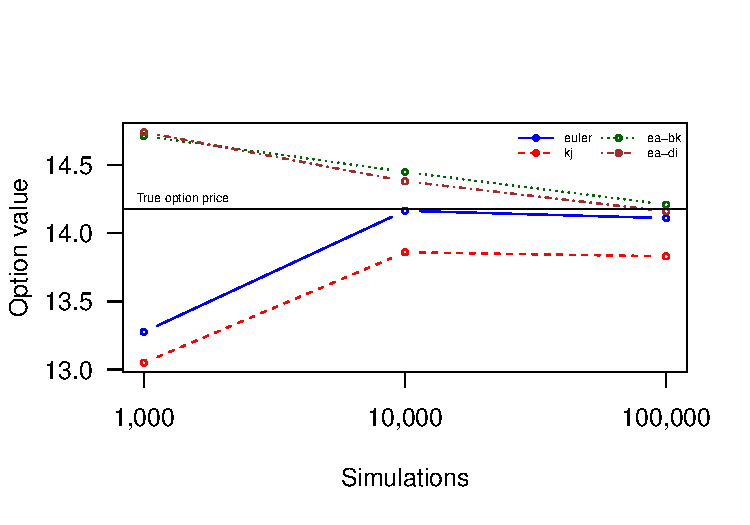
\includegraphics{thesis_files/figure-latex/modcomp11-1} 
  
  }
  
  \caption{Comparison between models, 20 steps. \label{modcomp1}}\label{fig:modcomp11}
  \end{figure}
  To verify if in fact these methods present bias, we performed ten
  thousand simulations of ten thousand paths to the Euler, Kahl-Jackel
  (KJ) and drift interpolated exact algorithm (EA-DI) with 20 steps
  (\(dt = 0.05\)) first. We present these results in appendix
  \ref{resultsapp} because we present the more precise simulations we
  made, with 100 steps in Figure \ref{fig:results10k001}. Results seem to
  show a little bias, thus we present in Table \ref{res2} how precise
  models are.
  \begin{figure}
  
  {\centering 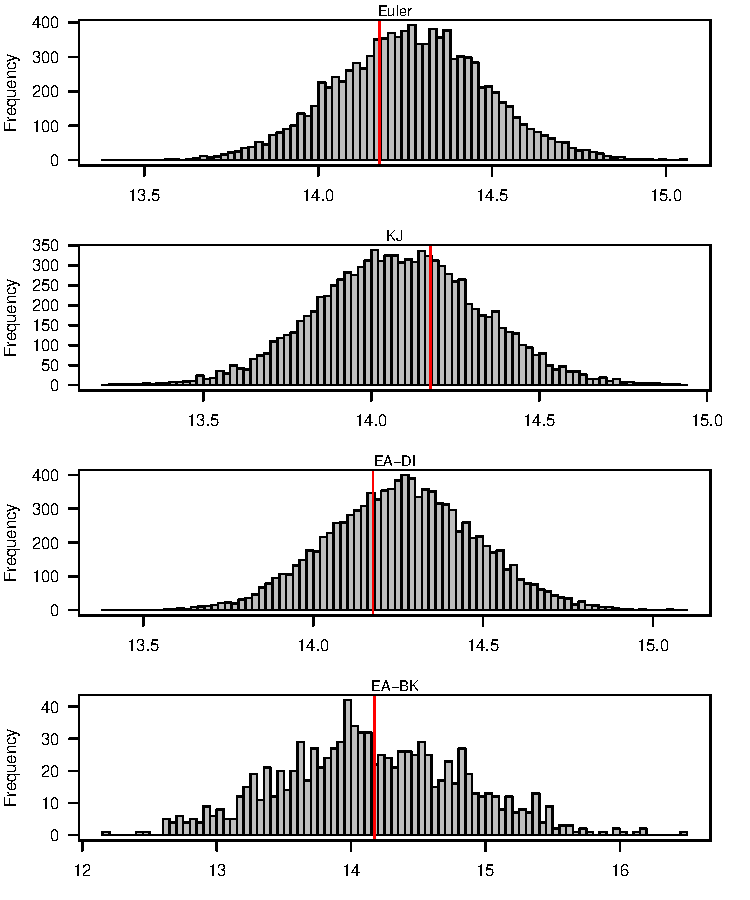
\includegraphics{thesis_files/figure-latex/results10k001-1} 
  
  }
  
  \caption{Comparison between models, 100 steps. \label{results10k001}}\label{fig:results10k001}
  \end{figure}
  The exact algorithm performs much slowlier than the other three we only
  performed 1000 simulations of one thousand paths each. That is why its
  RMSE is comparably bigger than the other three implementations. We are
  aware that, by construction the Broadie-Kaya version of the algorithm
  has no bias, but we tested the bias of our implementation (even though
  we didn't put it in the Table \ref{res2}) and the reason is twofold:
  again, we wanted to check if we correctly implemented the algorithm as a
  whole, but more importantly we wanted to check the outcomes of the
  adaptations we made (in terms of truncation, relative error and others)
  were playing into our model. The computed, even with far less
  simulations was far smaller than the other three methods, with only
  \(-0.02\). We understand that this result confirms that our adaptations
  did not change the nature of the model and with a greater number of
  simulations the bias would be zero as it should. We observe bias level
  in the three classical numerical models, the KJ model undervaluing in
  the same order (0.09) as the other two overvalue the option. In terms of
  standard deviation the models seem to be equivalent, with the KJ model
  presenting a slightly bigger standard deviation than the other two (0.24
  against 0.21 and 0.22). According to the tests performed, we are
  confident that our models were implemented correctly.
  \begin{table}[t]
  \centering
  \begin{tabular}{lrrrr}
    \hline 
   & Euler & KJ & EA-BK & EA-DI \\ 
    \hline 
  bias & 0.09 & -0.09 & - & 0.09 \\ 
    sd & 0.21 & 0.24 & - & 0.22 \\ 
    RMSE & 0.23 & 0.26 & 0.68 & 0.23 \\ 
     \hline 
  \multicolumn{5}{l}{\scriptsize{Note: Simulations performed with 100 steps, except the EA BK}} 
  \end{tabular}
  \caption{Estimators} 
  \label{res2}
  \end{table}
  \chapter{Conclusion}\label{conclusao}
  
  As we revisit what was presented through this thesis, we highlight that
  we were unable find codes of the heston's exact algorithm in any shape
  or form. That means we searched if the algorithm implementation was
  available in any programming language, or at least a reference to where
  to find it and we couldn't.
  
  Firstly, we provided a succint, but rigorous, theoretical framework.
  Since this topic is very embracing, we provided an abundant amount of
  literature not only to the core topics approached, but also to the
  marginal ones. The first topic introduced in our review of literature is
  the stochastic calculus subject. Following the basics, we present the
  Black-Scholes model since this is the basic model from which the
  stochastic volatility ones derive from. We show how the BS formula is
  computed, and its limitations. The next logical step are the stochastic
  volatility models since they directly attack and solve the biggest BS
  model limitation: fixed volatility. We present the CIR before the Heston
  model as the first concocts the latter. Lastly, approach the challenges
  brought by the adoption of numerical methods, to better understand if a
  method is theoretically good, how to perform a discretization, and why a
  supposedly good discretization scheme can fail, nevertheless.
  
  Thereafter, we thoroughly introduced the algorithms we were going to
  implement in R, and how we were going to do it. Four different
  algorithms were presented: the Euler scheme, the Kahl-Jackel algorithm,
  and two versions of the ``exact algorithm''. The first trying to be as
  similar as possible to the one presented in Broadie-Kaya's paper and the
  modified version bringing an approximation to the algorithm's second
  step (the costlier step) as we replace the integral with a drift
  interpolation.
  
  We tested the implementations and presented our results in Chapter
  @ref(\#resultados). We used a specification provided in Broadie-Kaya's
  paper {[}31{]}, Table 2 with two slight changes. We reduced the time to
  maturity from 5 to 1 year and we reduced the \(\sigma\) from 1 to 0.2
  following the rules he acknowledges and previously cited. We verified
  that, in fact, the EA algorithm does not present bias, but because of
  the nature of the algorithm and of the implementation in R, we doubt it
  can be used practically without finding a way around the algorithm's
  second step.
  
  As we performed the EA's implementation we faced some challenges we
  weren't able to resolve yet. We couldn't parallelize the root inversion,
  which was a big bottleneck for the algorithm that we will solve. Also,
  we only created methods for the European \emph{call} and for four
  different schemes. We intend to widen the scope to embrace the
  \emph{put} computation and introduce the binomial tree approach along
  with the method of moments and maximum likelihood. Finally, the package
  with all its functions is available at this
  \href{<https://github.com/fernote7/rnmethods>}{\textbf{link}}\footnote{\url{https://github.com/fernote7/rnmethods}}
  and in the near future on
  \href{<https://cran.r-project.org/>}{\textbf{CRAN}}.
  
  \appendix
  
  \chapter{Black-Scholes formula}\label{bsformula}
  
  In this appendix, we start from the following Geometric Brownian Motion
  process:
  \begin{align*}
  dS_t &= \mu S_t dt + \sigma S_t dB_t
  \end{align*}
  And we claim that the solution to this stochastic differential equation
  applying Itô's calculus is the following formula:
  \begin{align*}
  S_T &= S_0 \times \exp \left( \left( \mu  - \frac{\sigma^2}{2} \right) T  + \sigma B_T \right)
  \end{align*}
  \begin{proof}
  
  If $S$ were deterministic, $dS_t/S_t$ would be the derivative of $\ln(S_t)$ with respect to $S$. This suggests to find an expression for the stochastic differential of $\ln(S_t)$, a function of the single random variable $S_t$.
  
  
  \begin{align*} 
  f(t,S) &= \ln(S) \\[10pt]
  df(t,S) &= \frac{\partial f}{\partial S} dS + \frac{1}{2} \frac{\partial^2 f}{\partial S^2} (dS)^2 \\[10pt]
  d\ln(S) &= \frac{d\ln(S)}{dS} dS + \frac{1}{2} \frac{d^2\ln(S)}{dS^2}(dS)^2 \\[10pt]
  (dS)^2 &= \int_{0}^{t}{\left(\sigma \times S \right)^2} ds = \sigma^2 S^2 dt \\[10pt]
  d\ln(S) &= \frac{1}{S} (\mu S dt + \sigma S dB) + \frac{1}{2}\frac{-1}{S^2} \sigma^2 S^2 dt \\[10pt]
  d\ln(S) &= \left( \mu -  \frac{1}{2} \sigma^2 \right) dt + \sigma dB \\[10pt]
  \int_{t=0}^{T}{d\ln(S_T)} &= \int_{t=0}^{T}{\left( \mu - \frac{\sigma^2}{2} \right) dt} + \int_{t=0}^{T}{\sigma dB_t} 
  \end{align*}
  \begin{align*} 
  \ln(S_T) - \ln(S_0) &=  \left(\mu  - \frac{\sigma^2}{2} \right)  T + \sigma B_T \\[10pt]
  \ln \left( \frac{S_T}{S_0} \right) &= \left( \mu  - \frac{\sigma^2}{2}  \right) T + \sigma B_T \\[10pt]
  S_T &= S_0 \times \exp \left( \left( \mu  - \frac{\sigma^2}{2} \right) T  + \sigma B_T \right) 
  \end{align*}
  \end{proof}
  \chapter{Bessel Function}\label{bessel}
  
  The modified Bessel function of the first kind can be described in the
  shape of a contour integral (below) and is plotted for three different
  \(\nu\) in Figure \ref{fig:bessel}.
  \begin{align*} 
  I_n(z)= \frac{1}{2 \pi i}\displaystyle \oint e^{(z/2)(t+1/t)}t^{-n-1}dt
  \end{align*}
  However, the Broadie-Kaya paper {[}31{]} presents it as a power series:
  \begin{align*}
  I_{\nu}(z)= \left(\frac{1}{2}z\right)^\nu \displaystyle \sum_{k=0}^{\infty}{\frac{\left(\frac{1}{4}z^2\right)^k}{\left(k!\Gamma \left(\nu+k+1\right)\right)}}
  \end{align*}
  With \(\Gamma(x)\) is the gamma function and \(\nu\) ia a complex
  number.
  \begin{figure}
  
  {\centering 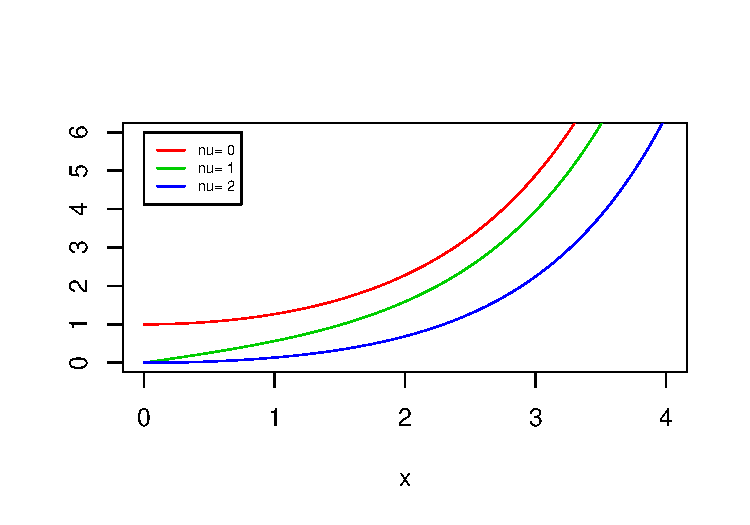
\includegraphics{thesis_files/figure-latex/bessel-1} 
  
  }
  
  \caption{Modified Bessel Functions of the First Kind \label{bessel}}\label{fig:bessel}
  \end{figure}
  \chapter{Implementations}\label{imps}
  
  \section{Euler Scheme}\label{eulerapp}
  
  \small
  \begin{Shaded}
  \begin{Highlighting}[]
  \NormalTok{hestoneuler <-}\StringTok{ }\ControlFlowTok{function}\NormalTok{(S, X, r, v, theta, rho, k, }
  \NormalTok{                        sigma, }\DataTypeTok{t =} \DecValTok{0}\NormalTok{, }\DataTypeTok{dt =} \OtherTok{NULL}\NormalTok{, }\DataTypeTok{tau =} \DecValTok{1}\NormalTok{, N)\{}
  
    \ControlFlowTok{if}\NormalTok{(}\KeywordTok{is.null}\NormalTok{(dt))\{ dt <-}\StringTok{ }\NormalTok{(tau}\OperatorTok{-}\NormalTok{t)}\OperatorTok{/}\DecValTok{1000}\NormalTok{\}}
  \NormalTok{  sequencia <-}\StringTok{ }\KeywordTok{seq}\NormalTok{(t,tau,dt)}
  \NormalTok{  ST <-}\StringTok{ }\KeywordTok{matrix}\NormalTok{(}\OtherTok{NA}\NormalTok{, }\KeywordTok{length}\NormalTok{(sequencia), N) }\CommentTok{#transformar em matrix}
  \NormalTok{  aux <-}\StringTok{ }\OtherTok{NULL}
  \NormalTok{  sqrt_dt <-}\StringTok{ }\KeywordTok{sqrt}\NormalTok{(dt)}
  
    \ControlFlowTok{for}\NormalTok{(i }\ControlFlowTok{in}\NormalTok{ sequencia)\{}
  \NormalTok{    Zv <-}\StringTok{ }\NormalTok{stats}\OperatorTok{::}\KeywordTok{rnorm}\NormalTok{(N)}
  \NormalTok{    Zt <-}\StringTok{ }\NormalTok{stats}\OperatorTok{::}\KeywordTok{rnorm}\NormalTok{(N)}
  \NormalTok{    Zs <-}\StringTok{ }\NormalTok{rho }\OperatorTok{*}\StringTok{ }\NormalTok{Zv }\OperatorTok{+}\StringTok{ }\NormalTok{(}\KeywordTok{sqrt}\NormalTok{(}\DecValTok{1} \OperatorTok{-}\StringTok{ }\NormalTok{(rho}\OperatorTok{^}\DecValTok{2}\NormalTok{)) }\OperatorTok{*}\StringTok{ }\NormalTok{Zt)}
  \NormalTok{    aux <-}\StringTok{ }\NormalTok{v}
  \NormalTok{    aux[v }\OperatorTok{<}\StringTok{ }\DecValTok{0}\NormalTok{] <-}\StringTok{ }\DecValTok{0}
  \NormalTok{    sqrt_aux <-}\StringTok{ }\KeywordTok{sqrt}\NormalTok{(aux)}
  \NormalTok{    S <-}\StringTok{ }\NormalTok{S }\OperatorTok{*}\StringTok{ }\NormalTok{(}\DecValTok{1} \OperatorTok{+}\StringTok{ }\NormalTok{r }\OperatorTok{*}\StringTok{ }\NormalTok{dt }\OperatorTok{+}\StringTok{ }\NormalTok{sqrt_aux }\OperatorTok{*}\StringTok{ }\NormalTok{Zs }\OperatorTok{*}\StringTok{ }\NormalTok{sqrt_dt)}
  \NormalTok{    S[S }\OperatorTok{<=}\StringTok{ }\DecValTok{0}\NormalTok{] =}\StringTok{ }\DecValTok{0}
  \NormalTok{    v <-}\StringTok{ }\NormalTok{v }\OperatorTok{+}\StringTok{ }\NormalTok{k }\OperatorTok{*}\StringTok{ }\NormalTok{dt }\OperatorTok{*}\StringTok{ }\NormalTok{(theta }\OperatorTok{-}\StringTok{ }\NormalTok{aux) }\OperatorTok{+}\StringTok{ }\NormalTok{sigma }\OperatorTok{*}\StringTok{ }\NormalTok{sqrt_aux }\OperatorTok{*}\StringTok{ }\NormalTok{Zv }\OperatorTok{*}\StringTok{ }\NormalTok{sqrt_dt}
  \NormalTok{    ST[j,] <-}\StringTok{ }\NormalTok{S}
  \NormalTok{  \}}
    \KeywordTok{rm}\NormalTok{(aux, v, Zv, Zt, Zs, S, j)}
  \NormalTok{  ST <-}\StringTok{ }\KeywordTok{as.matrix}\NormalTok{(ST, }\DataTypeTok{ncol=}\NormalTok{N)}
  \NormalTok{  Result <-}\StringTok{ }\NormalTok{ST[}\KeywordTok{nrow}\NormalTok{(ST),] }\OperatorTok{-}\StringTok{ }\NormalTok{X}
  \NormalTok{  Result[Result }\OperatorTok{<=}\StringTok{ }\DecValTok{0}\NormalTok{] =}\StringTok{ }\DecValTok{0}
  \NormalTok{  call =}\StringTok{ }\KeywordTok{mean}\NormalTok{(}\KeywordTok{exp}\NormalTok{(}\OperatorTok{-}\NormalTok{r}\OperatorTok{*}\NormalTok{(tau}\OperatorTok{-}\NormalTok{t))}\OperatorTok{*}\NormalTok{Result)}
  \NormalTok{  lista =}\StringTok{ }\KeywordTok{list}\NormalTok{(}\StringTok{'call'}\NormalTok{ =}\StringTok{ }\NormalTok{call, }\StringTok{'Result'}\NormalTok{ =}\StringTok{ }\NormalTok{Result, }\StringTok{'Spot'}\NormalTok{ =}\StringTok{ }\NormalTok{ST)}
    \KeywordTok{return}\NormalTok{(lista)}
  \NormalTok{\}}
  \end{Highlighting}
  \end{Shaded}
  \section{Kahl-Jackel Implementation}\label{kjimp}
  
  \footnotesize
  \begin{Shaded}
  \begin{Highlighting}[]
  \NormalTok{Hestoncallkj <-}\StringTok{ }\ControlFlowTok{function}\NormalTok{(S, X, r, q, v, theta, rho, k, }
  \NormalTok{                         sigma, }\DataTypeTok{t =} \DecValTok{0}\NormalTok{, }\DataTypeTok{dt =} \OtherTok{NULL}\NormalTok{, }\DataTypeTok{tau =} \DecValTok{1}\NormalTok{, N)\{}
  
      \ControlFlowTok{if}\NormalTok{(}\KeywordTok{is.null}\NormalTok{(dt))\{ dt <-}\StringTok{ }\NormalTok{(T}\OperatorTok{-}\NormalTok{t)}\OperatorTok{/}\DecValTok{1000}\NormalTok{\}}
  \NormalTok{    v <-}\StringTok{ }\KeywordTok{rep}\NormalTok{(v,N)}
  \NormalTok{    theta<-}\StringTok{ }\KeywordTok{rep}\NormalTok{(theta,N)}
  \NormalTok{    sequencia <-}\StringTok{ }\KeywordTok{seq}\NormalTok{(t,tau,dt)}
  \NormalTok{    ST <-}\StringTok{ }\KeywordTok{matrix}\NormalTok{(}\OtherTok{NA}\NormalTok{, }\KeywordTok{length}\NormalTok{(sequencia), N) }\CommentTok{#transformar em matrix}
  \NormalTok{    S <-}\StringTok{ }\KeywordTok{log}\NormalTok{(S)}
  
      \ControlFlowTok{for}\NormalTok{(i }\ControlFlowTok{in} \KeywordTok{seq}\NormalTok{(t,tau,dt))\{}
  \NormalTok{        Zv <-}\StringTok{ }\NormalTok{stats}\OperatorTok{::}\KeywordTok{rnorm}\NormalTok{(N)}
  \NormalTok{        Zt <-}\StringTok{ }\NormalTok{stats}\OperatorTok{::}\KeywordTok{rnorm}\NormalTok{(N)}
  \NormalTok{        Zs <-}\StringTok{ }\NormalTok{rho }\OperatorTok{*}\StringTok{ }\NormalTok{Zv }\OperatorTok{+}\StringTok{ }\KeywordTok{sqrt}\NormalTok{(}\DecValTok{1} \OperatorTok{-}\StringTok{ }\NormalTok{rho}\OperatorTok{^}\DecValTok{2}\NormalTok{) }\OperatorTok{*}\StringTok{ }\NormalTok{Zt}
  \NormalTok{        vt <-}\StringTok{ }\NormalTok{(v }\OperatorTok{+}\StringTok{ }\NormalTok{k }\OperatorTok{*}\StringTok{ }\NormalTok{theta }\OperatorTok{*}\StringTok{ }\NormalTok{dt }\OperatorTok{+}\StringTok{ }\NormalTok{sigma }\OperatorTok{*}\StringTok{ }\KeywordTok{sqrt}\NormalTok{(v) }\OperatorTok{*}\StringTok{ }\NormalTok{Zv }\OperatorTok{*}\StringTok{ }\KeywordTok{sqrt}\NormalTok{(dt) }\OperatorTok{+}
  \StringTok{                  }\NormalTok{(}\DecValTok{1}\OperatorTok{/}\DecValTok{4}\NormalTok{) }\OperatorTok{*}\StringTok{ }\NormalTok{sigma}\OperatorTok{^}\DecValTok{2} \OperatorTok{*}\StringTok{ }\NormalTok{dt }\OperatorTok{*}\StringTok{ }\NormalTok{((Zv)}\OperatorTok{^}\DecValTok{2} \OperatorTok{-}\StringTok{ }\DecValTok{1}\NormalTok{))}\OperatorTok{/}\NormalTok{(}\DecValTok{1} \OperatorTok{+}\StringTok{ }\NormalTok{k }\OperatorTok{*}\StringTok{ }\NormalTok{dt)}
  \NormalTok{        vt[vt }\OperatorTok{<=}\StringTok{ }\DecValTok{0}\NormalTok{] <-}\StringTok{ }\NormalTok{v[vt }\OperatorTok{<=}\StringTok{ }\DecValTok{0}\NormalTok{] }\OperatorTok{+}\StringTok{ }\NormalTok{k }\OperatorTok{*}\StringTok{ }\NormalTok{dt }\OperatorTok{*}\StringTok{ }\NormalTok{(theta[vt }\OperatorTok{<=}\StringTok{ }\DecValTok{0}\NormalTok{] }\OperatorTok{-}\StringTok{ }
  \StringTok{                        }\NormalTok{v[vt }\OperatorTok{<=}\StringTok{ }\DecValTok{0}\NormalTok{],}\DecValTok{0}\NormalTok{) }\OperatorTok{+}\StringTok{ }\NormalTok{sigma }\OperatorTok{*}\StringTok{ }\KeywordTok{sqrt}\NormalTok{(v[vt }\OperatorTok{<=}\StringTok{ }\DecValTok{0}\NormalTok{],}\DecValTok{0}\NormalTok{) }\OperatorTok{*}\StringTok{ }
  \StringTok{                        }\NormalTok{Zv[vt }\OperatorTok{<=}\StringTok{ }\DecValTok{0}\NormalTok{] }\OperatorTok{*}\StringTok{ }\KeywordTok{sqrt}\NormalTok{(dt)}
  \NormalTok{        v <-}\StringTok{ }\NormalTok{vt}
  \NormalTok{        v[v}\OperatorTok{<=}\DecValTok{0}\NormalTok{] <-}\StringTok{ }\DecValTok{0}
  \NormalTok{        vt[vt}\OperatorTok{<=}\DecValTok{0}\NormalTok{] <-}\StringTok{ }\DecValTok{0}
  \NormalTok{        S <-}\StringTok{ }\NormalTok{S }\OperatorTok{+}\StringTok{ }\NormalTok{(r }\OperatorTok{-}\StringTok{ }\NormalTok{(v}\OperatorTok{+}\NormalTok{vt)}\OperatorTok{/}\DecValTok{4}\NormalTok{) }\OperatorTok{*}\StringTok{ }\NormalTok{dt }\OperatorTok{+}\StringTok{ }\NormalTok{rho }\OperatorTok{*}\StringTok{ }\KeywordTok{sqrt}\NormalTok{(v) }\OperatorTok{*}\StringTok{ }\NormalTok{Zv }\OperatorTok{*}\StringTok{ }\KeywordTok{sqrt}\NormalTok{(dt) }\OperatorTok{+}
  \StringTok{             }\NormalTok{(}\DecValTok{1}\OperatorTok{/}\DecValTok{2}\NormalTok{) }\OperatorTok{*}\StringTok{ }\NormalTok{(}\KeywordTok{sqrt}\NormalTok{(v) }\OperatorTok{+}\StringTok{ }\KeywordTok{sqrt}\NormalTok{(vt)) }\OperatorTok{*}\StringTok{ }\NormalTok{(Zs }\OperatorTok{+}\StringTok{ }\NormalTok{rho }\OperatorTok{*}\StringTok{ }\NormalTok{Zv) }\OperatorTok{*}\StringTok{ }\KeywordTok{sqrt}\NormalTok{(dt) }\OperatorTok{+}
  \StringTok{             }\NormalTok{((rho }\OperatorTok{*}\StringTok{ }\NormalTok{sigma }\OperatorTok{*}\StringTok{ }\NormalTok{dt)}\OperatorTok{/}\DecValTok{2}\NormalTok{) }\OperatorTok{*}\StringTok{ }\NormalTok{((Zv)}\OperatorTok{^}\DecValTok{2} \OperatorTok{-}\StringTok{ }\DecValTok{1}\NormalTok{)}
  \NormalTok{        S[S }\OperatorTok{<=}\StringTok{ }\DecValTok{0}\NormalTok{] =}\StringTok{ }\DecValTok{0}
  \NormalTok{        ST[j,] <-}\StringTok{ }\NormalTok{S}
  \NormalTok{    \}}
  \NormalTok{    ST <-}\StringTok{ }\KeywordTok{as.matrix}\NormalTok{(ST, }\DataTypeTok{ncol=}\NormalTok{N)}
  \NormalTok{    Result <-}\StringTok{ }\KeywordTok{exp}\NormalTok{(ST[}\KeywordTok{nrow}\NormalTok{(ST),]) }\OperatorTok{-}\StringTok{ }\NormalTok{X}
  \NormalTok{    Result[Result }\OperatorTok{<=}\StringTok{ }\DecValTok{0}\NormalTok{] =}\StringTok{ }\DecValTok{0}
  \NormalTok{    call =}\StringTok{ }\KeywordTok{mean}\NormalTok{(}\KeywordTok{exp}\NormalTok{(}\OperatorTok{-}\NormalTok{r}\OperatorTok{*}\NormalTok{tau)}\OperatorTok{*}\NormalTok{Result)}
  
  \NormalTok{    lista =}\StringTok{ }\KeywordTok{list}\NormalTok{(}\StringTok{'call'}\NormalTok{ =}\StringTok{ }\NormalTok{call, }\StringTok{'Result'}\NormalTok{ =}\StringTok{ }\NormalTok{Result, }\StringTok{'Spot'}\NormalTok{ =}\StringTok{ }\NormalTok{ST)}
      \KeywordTok{return}\NormalTok{(lista)}
  \NormalTok{\}}
  \end{Highlighting}
  \end{Shaded}
  \section{Exact Algorithm}\label{eabk}
  
  \footnotesize
  \begin{Shaded}
  \begin{Highlighting}[]
  \NormalTok{phi_heston <-}\StringTok{ }\ControlFlowTok{function}\NormalTok{(a, v0, v_t, d)\{}
  
  \NormalTok{    gamma_a <-}\StringTok{ }\KeywordTok{sqrt}\NormalTok{(k}\OperatorTok{^}\DecValTok{2} \OperatorTok{-}\StringTok{ }\DecValTok{2} \OperatorTok{*}\StringTok{ }\NormalTok{sigma}\OperatorTok{^}\DecValTok{2} \OperatorTok{*}\StringTok{ }\NormalTok{1i}\OperatorTok{*}\NormalTok{a)}
  \NormalTok{    gammadt <-}\StringTok{ }\NormalTok{gamma_a }\OperatorTok{*}\StringTok{ }\NormalTok{(tau}\OperatorTok{-}\NormalTok{t)}
  \NormalTok{    sqrtv0vt <-}\StringTok{ }\KeywordTok{sqrt}\NormalTok{(v0}\OperatorTok{*}\NormalTok{v_t)}
  \NormalTok{    delta <-}\StringTok{ }\OperatorTok{-}\NormalTok{k }\OperatorTok{*}\StringTok{ }\NormalTok{(tau}\OperatorTok{-}\NormalTok{t)}
  
  \NormalTok{    part1 <-}\StringTok{ }\NormalTok{(gamma_a }\OperatorTok{*}\StringTok{ }\KeywordTok{exp}\NormalTok{(}\OperatorTok{-}\NormalTok{(gamma_a }\OperatorTok{-}\StringTok{ }\NormalTok{k)}\OperatorTok{/}\DecValTok{2} \OperatorTok{*}\StringTok{ }\NormalTok{(tau}\OperatorTok{-}\NormalTok{t)) }\OperatorTok{*}\StringTok{ }\NormalTok{(}\DecValTok{1} \OperatorTok{-}\StringTok{ }\KeywordTok{exp}\NormalTok{(delta)))}\OperatorTok{/}
  \StringTok{        }\NormalTok{(k }\OperatorTok{*}\StringTok{ }\NormalTok{(}\DecValTok{1}\OperatorTok{-}\StringTok{ }\KeywordTok{exp}\NormalTok{(}\OperatorTok{-}\StringTok{ }\NormalTok{gammadt)))}
  
  \NormalTok{    part2 <-}\StringTok{ }\KeywordTok{exp}\NormalTok{((v0}\OperatorTok{+}\NormalTok{v_t)}\OperatorTok{/}\NormalTok{(sigma}\OperatorTok{^}\DecValTok{2}\NormalTok{) }\OperatorTok{*}\StringTok{ }\NormalTok{( (k }\OperatorTok{*}\StringTok{ }\NormalTok{(}\DecValTok{1} \OperatorTok{+}\StringTok{ }\KeywordTok{exp}\NormalTok{(delta)))}\OperatorTok{/}\NormalTok{(}\DecValTok{1}\OperatorTok{-}\KeywordTok{exp}\NormalTok{(delta)) }\OperatorTok{-}
  \StringTok{                        }\NormalTok{(gamma_a }\OperatorTok{*}\StringTok{ }\NormalTok{(}\DecValTok{1} \OperatorTok{+}\StringTok{ }\KeywordTok{exp}\NormalTok{(}\OperatorTok{-}\StringTok{ }\NormalTok{gammadt)))}\OperatorTok{/}\NormalTok{(}\DecValTok{1}\OperatorTok{-}\KeywordTok{exp}\NormalTok{(}\OperatorTok{-}\StringTok{ }\NormalTok{gammadt))))}
  
  \NormalTok{    part3 <-}\StringTok{ }\NormalTok{Bessel}\OperatorTok{::}\KeywordTok{BesselI}\NormalTok{(}\DataTypeTok{z =}\NormalTok{ ((}\DecValTok{4} \OperatorTok{*}\StringTok{ }\NormalTok{gamma_a }\OperatorTok{*}\StringTok{ }\NormalTok{sqrtv0vt)}\OperatorTok{/}\NormalTok{(sigma}\OperatorTok{^}\DecValTok{2}\NormalTok{) }\OperatorTok{*}
  \StringTok{                                      }\KeywordTok{exp}\NormalTok{(}\OperatorTok{-}\StringTok{ }\NormalTok{gammadt}\OperatorTok{/}\DecValTok{2}\NormalTok{)}\OperatorTok{/}
  \StringTok{                                      }\NormalTok{(}\DecValTok{1} \OperatorTok{-}\StringTok{ }\KeywordTok{exp}\NormalTok{(}\OperatorTok{-}\StringTok{ }\NormalTok{gammadt))), }\DataTypeTok{nu =} \FloatTok{0.5}\OperatorTok{*}\NormalTok{d }\OperatorTok{-}\StringTok{ }\DecValTok{1}\NormalTok{) }\OperatorTok{/}
  \StringTok{        }\NormalTok{Bessel}\OperatorTok{::}\KeywordTok{BesselI}\NormalTok{(}\DataTypeTok{z =}\NormalTok{ ((}\DecValTok{4} \OperatorTok{*}\StringTok{ }\NormalTok{k }\OperatorTok{*}\StringTok{ }\NormalTok{sqrtv0vt)}\OperatorTok{/}\NormalTok{(sigma}\OperatorTok{^}\DecValTok{2}\NormalTok{) }\OperatorTok{*}\StringTok{ }\NormalTok{(}\KeywordTok{exp}\NormalTok{(delta}\OperatorTok{/}\DecValTok{2}\NormalTok{))}\OperatorTok{/}
  \StringTok{                                 }\NormalTok{(}\DecValTok{1}\OperatorTok{-}\KeywordTok{exp}\NormalTok{(delta))), }\DataTypeTok{nu =} \FloatTok{0.5}\OperatorTok{*}\NormalTok{d }\OperatorTok{-}\StringTok{ }\DecValTok{1}\NormalTok{)}
  
      \KeywordTok{return}\NormalTok{ (part1 }\OperatorTok{*}\StringTok{ }\NormalTok{part2 }\OperatorTok{*}\StringTok{ }\NormalTok{part3)}
  \NormalTok{\}}
  
  
  
  \NormalTok{intv <-}\StringTok{ }\ControlFlowTok{function}\NormalTok{(n, cf, v_t)\{}
  \NormalTok{    integrand <-}\StringTok{ }\ControlFlowTok{function}\NormalTok{(x, }\DataTypeTok{phi =}\NormalTok{ cf)\{}
  
  \NormalTok{        f2 <-}\StringTok{ }\ControlFlowTok{function}\NormalTok{(u)\{}
              \KeywordTok{Im}\NormalTok{(}\KeywordTok{phi}\NormalTok{(u) }\OperatorTok{*}\StringTok{ }\KeywordTok{exp}\NormalTok{(}\OperatorTok{-}\NormalTok{1i }\OperatorTok{*}\StringTok{ }\NormalTok{u }\OperatorTok{*}\StringTok{ }\NormalTok{x)) }\OperatorTok{/}\NormalTok{u}
  \NormalTok{        \}}
          \KeywordTok{return}\NormalTok{(f2)}
  \NormalTok{    \}}
  
  \NormalTok{    ## integrate to "cdf"}
  \NormalTok{    F_x <-}\StringTok{ }\ControlFlowTok{function}\NormalTok{ (x) \{}
  \NormalTok{        y <-}\StringTok{ }\FloatTok{0.5} \OperatorTok{-}\StringTok{ }\DecValTok{1}\OperatorTok{/}\NormalTok{pi }\OperatorTok{*}\StringTok{ }\KeywordTok{integrate}\NormalTok{(}\KeywordTok{integrand}\NormalTok{(x),  }\DataTypeTok{lower=} \DecValTok{0}\NormalTok{, }\DataTypeTok{upper=} \DecValTok{1000}\NormalTok{,}
                                      \DataTypeTok{rel.tol =} \FloatTok{0.001}\NormalTok{, }\DataTypeTok{stop.on.error =} \OtherTok{FALSE}\NormalTok{)}\OperatorTok{$}\NormalTok{value}
          \KeywordTok{return}\NormalTok{(y)}
  \NormalTok{    \}}
  
  \NormalTok{    ## endsign}
  
  \NormalTok{    endsign <-}\StringTok{ }\ControlFlowTok{function}\NormalTok{(f, }\DataTypeTok{sign =} \DecValTok{1}\NormalTok{) \{}
  \NormalTok{        b <-}\StringTok{ }\NormalTok{sign}
          \ControlFlowTok{while}\NormalTok{ (sign }\OperatorTok{*}\StringTok{ }\KeywordTok{f}\NormalTok{(b) }\OperatorTok{<}\StringTok{ }\DecValTok{0}\NormalTok{) b <-}\StringTok{ }\DecValTok{10} \OperatorTok{*}\StringTok{ }\NormalTok{b}
          \KeywordTok{return}\NormalTok{(b)}
  \NormalTok{    \}}
  
  \NormalTok{    ## inversion}
  
  \NormalTok{    low_bound =}\StringTok{ }\OperatorTok{-}\OtherTok{Inf}
  \NormalTok{    upp_bound =}\StringTok{ }\OtherTok{Inf}
  \NormalTok{    invcdf <-}\StringTok{ }\ControlFlowTok{function}\NormalTok{(u) \{}
  \NormalTok{        subcdf <-}\StringTok{ }\ControlFlowTok{function}\NormalTok{(t) }\KeywordTok{F_x}\NormalTok{(t) }\OperatorTok{-}\StringTok{ }\NormalTok{u}
          \ControlFlowTok{if}\NormalTok{ (low_bound }\OperatorTok{==}\StringTok{ }\OperatorTok{-}\OtherTok{Inf}\NormalTok{)}
  \NormalTok{            low_bound <-}\StringTok{ }\KeywordTok{endsign}\NormalTok{(subcdf, }\OperatorTok{-}\DecValTok{1}\NormalTok{)}
          \ControlFlowTok{if}\NormalTok{ (upp_bound }\OperatorTok{==}\StringTok{ }\OtherTok{Inf}\NormalTok{)}
  \NormalTok{            upp_bound <-}\StringTok{ }\KeywordTok{endsign}\NormalTok{(subcdf)}
          \KeywordTok{return}\NormalTok{(}\KeywordTok{uniroot}\NormalTok{(subcdf, }\DataTypeTok{lower=}\NormalTok{low_bound, }\DataTypeTok{upper=}\NormalTok{upp_bound, }
                         \DataTypeTok{tol =} \FloatTok{0.001220703}\NormalTok{)}\OperatorTok{$}\NormalTok{root)}
  \NormalTok{    \}}
  \NormalTok{    U <-}\StringTok{ }\NormalTok{stats}\OperatorTok{::}\KeywordTok{runif}\NormalTok{(n)}
      \KeywordTok{sapply}\NormalTok{(U, invcdf)}
  \NormalTok{\}}
  
  \NormalTok{hestonea_mod <-}\StringTok{ }\ControlFlowTok{function}\NormalTok{(S, X, r, v, theta, rho, k, sigma, }\DataTypeTok{t =} \DecValTok{0}\NormalTok{, }\DataTypeTok{tau =} \DecValTok{1}\NormalTok{)\{}
  
  \NormalTok{    d1 <-}\StringTok{ }\NormalTok{(}\DecValTok{4} \OperatorTok{*}\StringTok{ }\NormalTok{k }\OperatorTok{*}\StringTok{ }\NormalTok{theta)}\OperatorTok{/}\NormalTok{(sigma)}\OperatorTok{^}\DecValTok{2}
  \NormalTok{    c0 <-}\StringTok{ }\NormalTok{(sigma}\OperatorTok{^}\DecValTok{2} \OperatorTok{*}\StringTok{ }\NormalTok{(}\DecValTok{1} \OperatorTok{-}\StringTok{ }\KeywordTok{exp}\NormalTok{(}\OperatorTok{-}\NormalTok{k}\OperatorTok{*}\NormalTok{tau)))}\OperatorTok{/}\NormalTok{(}\DecValTok{4}\OperatorTok{*}\NormalTok{k)}
  \NormalTok{    dt <-}\StringTok{ }\NormalTok{(tau}\OperatorTok{-}\NormalTok{t)}
  \NormalTok{    ST <-}\StringTok{ }\OtherTok{NULL}
  
      \CommentTok{# sampling V}
  
  \NormalTok{    lambda <-}\StringTok{ }\NormalTok{(}\DecValTok{4}\OperatorTok{*}\NormalTok{k}\OperatorTok{*}\KeywordTok{exp}\NormalTok{(}\OperatorTok{-}\NormalTok{k}\OperatorTok{*}\NormalTok{dt)}\OperatorTok{*}\NormalTok{v)}\OperatorTok{/}\NormalTok{(sigma}\OperatorTok{^}\DecValTok{2} \OperatorTok{*}\StringTok{ }\NormalTok{(}\DecValTok{1}\OperatorTok{-}\KeywordTok{exp}\NormalTok{(}\OperatorTok{-}\NormalTok{k}\OperatorTok{*}\NormalTok{dt)))}
  \NormalTok{    vt <-}\StringTok{ }\NormalTok{c0 }\OperatorTok{*}\StringTok{ }\NormalTok{stats}\OperatorTok{::}\KeywordTok{rchisq}\NormalTok{(}\DataTypeTok{n =} \DecValTok{1}\NormalTok{, }\DataTypeTok{df =}\NormalTok{ d1, }\DataTypeTok{ncp =}\NormalTok{ lambda)}
  
      \CommentTok{# Sampling int\{V\}}
  
  \NormalTok{    phi <-}\StringTok{ }\ControlFlowTok{function}\NormalTok{(a, }\DataTypeTok{v0=}\NormalTok{v, }\DataTypeTok{v_t=}\NormalTok{vt, }\DataTypeTok{d=}\NormalTok{d1)\{}\KeywordTok{phi_heston}\NormalTok{(a, }\DataTypeTok{v0=}\NormalTok{v, }\DataTypeTok{v_t=}\NormalTok{vt, }\DataTypeTok{d=}\NormalTok{d1)\}}
      
  \NormalTok{    int_v <-}\StringTok{ }\KeywordTok{intv}\NormalTok{(}\DecValTok{1}\NormalTok{, }\DataTypeTok{cf =}\NormalTok{ phi, }\DataTypeTok{v_t=}\NormalTok{vt)}
      \CommentTok{# OR if you perform the drift interpolation scheme:}
      \CommentTok{#  int_v <- dt * ((1/2) * v + (1/2) * vt)}
      
      
      \CommentTok{# Sampling int\{v\}dw}
  \NormalTok{    int_vdw <-}\StringTok{ }\NormalTok{(}\DecValTok{1}\OperatorTok{/}\NormalTok{sigma) }\OperatorTok{*}\StringTok{ }\NormalTok{(vt }\OperatorTok{-}\StringTok{ }\NormalTok{v }\OperatorTok{-}\StringTok{ }\NormalTok{k }\OperatorTok{*}\StringTok{ }\NormalTok{theta }\OperatorTok{*}\StringTok{ }\NormalTok{dt }\OperatorTok{+}\StringTok{ }\NormalTok{k  }\OperatorTok{*}\StringTok{ }\NormalTok{int_v)}
  
      \CommentTok{# Sampling S}
      \ControlFlowTok{if}\NormalTok{( int_v }\OperatorTok{>=}\StringTok{ }\DecValTok{0}\NormalTok{)\{}
  \NormalTok{        m <-}\StringTok{ }\KeywordTok{log}\NormalTok{(S) }\OperatorTok{+}\StringTok{ }\NormalTok{(r }\OperatorTok{*}\StringTok{ }\NormalTok{(tau }\OperatorTok{-}\StringTok{ }\NormalTok{t) }\OperatorTok{-}\StringTok{ }\NormalTok{(}\DecValTok{1}\OperatorTok{/}\DecValTok{2}\NormalTok{) }\OperatorTok{*}\StringTok{ }\NormalTok{int_v }\OperatorTok{+}\StringTok{ }\NormalTok{rho }\OperatorTok{*}\StringTok{ }\NormalTok{int_vdw)}
  \NormalTok{        std <-}\StringTok{ }\KeywordTok{sqrt}\NormalTok{((}\DecValTok{1} \OperatorTok{-}\StringTok{ }\NormalTok{rho}\OperatorTok{^}\DecValTok{2}\NormalTok{)) }\OperatorTok{*}\StringTok{ }\KeywordTok{sqrt}\NormalTok{(int_v)}
  \NormalTok{        S <-}\StringTok{ }\KeywordTok{exp}\NormalTok{(m }\OperatorTok{+}\StringTok{ }\NormalTok{std }\OperatorTok{*}\StringTok{ }\KeywordTok{rnorm}\NormalTok{(}\DecValTok{1}\NormalTok{))}
  \NormalTok{        v <-}\StringTok{ }\NormalTok{vt}
  \NormalTok{        ST <-}\StringTok{ }\NormalTok{S}
  \NormalTok{    \} }\ControlFlowTok{else}\NormalTok{ \{}
  \NormalTok{        v <-}\StringTok{ }\NormalTok{vt}
  \NormalTok{        ST <-}\StringTok{ }\KeywordTok{rbind}\NormalTok{(ST,}\OtherTok{NA}\NormalTok{)\}}
  
  \NormalTok{    Result <-}\StringTok{ }\NormalTok{ST }\OperatorTok{-}\StringTok{ }\NormalTok{X}
  \NormalTok{    Result[Result }\OperatorTok{<=}\StringTok{ }\DecValTok{0}\NormalTok{] =}\StringTok{ }\DecValTok{0}
  \NormalTok{    call =}\StringTok{ }\KeywordTok{exp}\NormalTok{(}\OperatorTok{-}\NormalTok{r}\OperatorTok{*}\NormalTok{tau)}\OperatorTok{*}\NormalTok{Result}
  \NormalTok{    lista =}\StringTok{ }\KeywordTok{list}\NormalTok{(}\StringTok{'call'}\NormalTok{ =}\StringTok{ }\NormalTok{call, }\StringTok{'Result'}\NormalTok{ =}\StringTok{ }\NormalTok{Result, }\StringTok{'Spot'}\NormalTok{ =}\StringTok{ }\NormalTok{ST)}
      \KeywordTok{return}\NormalTok{(lista)}
  \NormalTok{\}}
  \end{Highlighting}
  \end{Shaded}
  \section{Results with 20 steps}\label{resultsapp}
  \begin{figure}
  
  {\centering 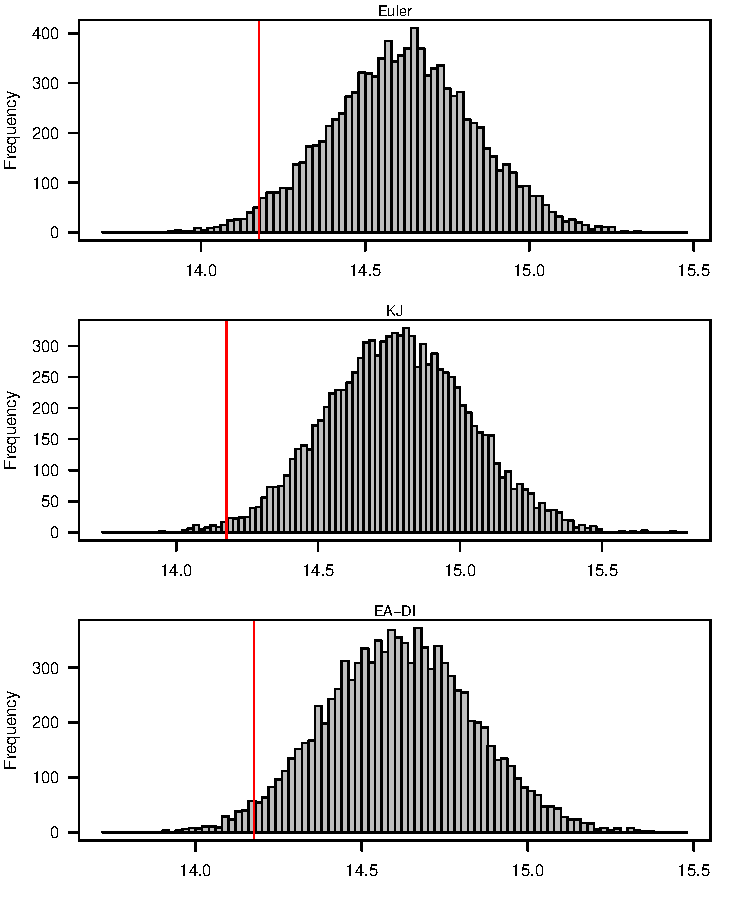
\includegraphics{thesis_files/figure-latex/results10k-1} 
  
  }
  
  \caption{Comparison between models, 20 steps. \label{results10k}}\label{fig:results10k}
  \end{figure}
  \normalsize
  
  \clearpage
  
  \fancyhead[L]{\slshape References} \fancyhead[R]{\slshape }
  
  \backmatter
  
  \chapter*{References}\label{references}
  \addcontentsline{toc}{chapter}{References}
  
  \setlength{\parindent}{-0.0in} \setlength{\leftskip}{0.00in}
  \setlength{\parskip}{8pt}
  
  \hypertarget{refs}{}
  \hypertarget{ref-black1973pricing}{}
  {[}1{]} Black, F.; Scholes, M. The pricing of options and corporate
  liabilities. Journal of political economy, v. 81, n. 3, p. 637--654,
  1973.
  
  \hypertarget{ref-rlang}{}
  {[}2{]} R Core Team. R: A language and environment for statistical
  computing. Vienna, Austria: 2017.
  
  \hypertarget{ref-ubbo}{}
  {[}3{]} Wiersema, U.F. Brownian motion calculus. 2008.
  
  \hypertarget{ref-karatzas2012brownian}{}
  {[}4{]} Karatzas, I.; Shreve, S. Brownian motion and stochastic
  calculus. 2012.
  
  \hypertarget{ref-helgadottir2016option}{}
  {[}5{]} Helgadóttir, A.D.; Ionescu, L. Option pricing within the heston
  model. 2016.
  
  \hypertarget{ref-evans}{}
  {[}6{]} Evans, L.C. An introduction to stochastic differential
  equations. 2012.
  
  \hypertarget{ref-rosenthal}{}
  {[}7{]} Rosenthal, J.S. A first look at rigorous probability theory.
  2006.
  
  \hypertarget{ref-tong2012option}{}
  Tong, Z. (2012). Option pricing with long memory stochastic volatility
  models.
  
  \hypertarget{ref-steele2012stochastic}{}
  {[}9{]} Steele, J.M. Stochastic calculus and financial applications.
  2012.
  
  \hypertarget{ref-ito1951}{}
  {[}10{]} Itō, K. On stochastic differential equations. 1951.
  
  \hypertarget{ref-ito1962}{}
  {[}11{]} Itô, K. The brownian motion and tensor fields on riemannian
  manifold. Proc. Int. Congr. Math., Stockholm, v. 2, 1962.
  
  \hypertarget{ref-yang2013valuing}{}
  {[}12{]} Yang, Y. Valuing a european option with the heston model. 2013.
  
  \hypertarget{ref-salomao2011precificaccao}{}
  {[}13{]} Salomão, M. de F. Precificação de opções financeiras: Um estudo
  sobre os modelos de black scholes e garch. 2011.
  
  \hypertarget{ref-merton1973theory}{}
  {[}14{]} Merton, R.C. Theory of rational option pricing. The Bell
  Journal of economics and management science, p. 141--183, 1973.
  
  \hypertarget{ref-tsay2005analysis}{}
  {[}15{]} Tsay, R.S. Analysis of financial time series. 2005.
  
  \hypertarget{ref-iacus2009simulation}{}
  {[}16{]} Iacus, S.M. Simulation and inference for stochastic
  differential equations: With r examples. 2009.
  
  \hypertarget{ref-krouglov2006intuitive}{}
  {[}17{]} Krouglov, A. Intuitive proof of black-scholes formula based on
  arbitrage and properties of lognormal distribution. arXiv preprint
  physics/0612022, 2006.
  
  \hypertarget{ref-nmof}{}
  {[}18{]} Gilli, M.; Maringer, D.; et al. Numerical methods and
  optimization in finance. Waltham, MA, USA: 2011.
  
  \hypertarget{ref-cox1985theory}{}
  {[}19{]} Cox, J.C.; Ingersoll Jr, J.E.; et al. A theory of the term
  structure of interest rates. Econometrica: Journal of the Econometric
  Society, p. 385--407, 1985.
  
  \hypertarget{ref-heston1993closed}{}
  {[}20{]} Heston, S.L. A closed-form solution for options with stochastic
  volatility with applications to bond and currency options. Review of
  financial studies, v. 6, n. 2, p. 327--343, 1993.
  
  \hypertarget{ref-gilli_numerical_2011}{}
  {[}21{]} Gilli, M.; Maringer, D.; et al. Numerical methods and
  optimization in finance. 2011.
  
  \hypertarget{ref-kloeden1992}{}
  {[}22{]} Kloeden, P.E.; Platen, E. Numerical solution of stochastic
  differential equations springer-verlag. 1992.
  
  \hypertarget{ref-gard1988}{}
  {[}23{]} Gard, T.C. Introduction to stochastic differential equations.
  1988.
  
  \hypertarget{ref-higham2001}{}
  {[}24{]} Higham, D.J. An algorithmic introduction to numerical
  simulation of stochastic differential equations. SIAM review, v. 43, n.
  3, p. 525--546, 2001.
  
  \hypertarget{ref-clements1973well}{}
  {[}25{]} Clements, D.; Anderson, B. Well-behaved itô equations with
  simulations that always misbehave. IEEE Transactions on Automatic
  Control, v. 18, n. 6, p. 676--677, 1973.
  
  \hypertarget{ref-clark1980maximum}{}
  {[}26{]} Clark, J.M., Cameron, R. The maximum rate of convergence of
  discrete approximations for stochastic differential equations. In:
  Stochastic differential systems filtering and control. 1980, p.
  162--171.
  
  \hypertarget{ref-kiusalaas2013numerical}{}
  {[}27{]} Kiusalaas, J. Numerical methods in engineering with python 3.
  2013.
  
  \hypertarget{ref-iserles}{}
  {[}28{]} Iserles, A. A first course in the numerical analysis of
  differential equations. 2009.
  
  \hypertarget{ref-burden2001}{}
  {[}29{]} Burden, R.L.; Faires, J.D. Numerical analysis. 2001.
  Brooks/Cole, USA, 2001.
  
  \hypertarget{ref-lambers}{}
  {[}30{]} Lambers, J.V.; Sumner, A.C. Explorations in numerical analysis.
  University o California at Irvine, 2016.
  
  \hypertarget{ref-broadie2006exact}{}
  {[}31{]} Broadie, M.; Kaya, Ö. Exact simulation of stochastic volatility
  and other affine jump diffusion processes. Operations research, v. 54,
  n. 2, p. 217--231, 2006.
  
  \hypertarget{ref-andersen}{}
  {[}32{]} Andersen, L.B. Efficient simulation of the heston stochastic
  volatility model. 2007.
  
  \hypertarget{ref-kahl2006fast}{}
  {[}33{]} Kahl, C.; Jäckel, P. Fast strong approximation monte carlo
  schemes for stochastic volatility models. Quantitative Finance, v. 6, n.
  6, p. 513--536, 2006.
  
  \hypertarget{ref-dunn2014estimating}{}
  Dunn, R., Hauser, P., Seibold, T., \& Gong, H. (2014). Estimating option
  prices with heston's stochastic volatility model.
  
  \hypertarget{ref-scott1996}{}
  {[}35{]} Scott, L. Simulating a multi-factor term structure model over
  relatively long discrete time periods. In: Proceedings of the iafe first
  annual computational finance conference. 1996,
  
  \hypertarget{ref-willard1997}{}
  {[}36{]} Willard, G.A. Calculating prices and sensitivities for
  path-independent derivatives securities in multifactor models. The
  Journal of Derivatives, v. 5, n. 1, p. 45--61, 1997.
  
  \hypertarget{ref-romano1997}{}
  {[}37{]} Romano, M.; Touzi, N. Contingent claims and market completeness
  in a stochastic volatility model. Mathematical Finance, v. 7, n. 4, p.
  399--412, 1997.
  
  \hypertarget{ref-baldeaux}{}
  {[}38{]} Baldeaux, J.; Platen, E. Functionals of multidimensional
  diffusions with applications to finance. 2013.
  
  \hypertarget{ref-johnson1995}{}
  Johnson, N.L., Kotz, S., \& Balakrishnan, N. (1995). Continuous
  univariate distributions, vol. 2 of wiley series in probability and
  mathematical statistics: Applied probability and statistics.
  
  \hypertarget{ref-besselpkg}{}
  {[}40{]} Maechler, M. Bessel: Bessel -- bessel functions computations
  and approximations. 2013.
  
  \hypertarget{ref-feller1971introduction}{}
  {[}41{]} Feller, W. Introduction to the theory of probability and its
  applications, vol. 2. II (2. Ed.) New York: Wiley, 1971.
  
  \hypertarget{ref-gil1951note}{}
  {[}42{]} Gil-Pelaez, J. Note on the inversion theorem. Biometrika, v.
  38, n. 3-4, p. 481--482, 1951.
  
  \hypertarget{ref-van2010efficient}{}
  {[}43{]} Van Haastrecht, A.; Pelsser, A. Efficient, almost exact
  simulation of the heston stochastic volatility model. International
  Journal of Theoretical and Applied Finance, v. 13, n. 01, p. 1--43,
  2010.
  
  \hypertarget{ref-nmofpack}{}
  {[}44{]} Schumann, E. Numerical methods and optimization in finance
  (nmof) manual. package version 0.40-0). 2011--2016.


  % Index?

\end{document}
